\documentclass[8pt, a4paper, landscape, fleqn]{scrartcl}
\usepackage[utf8]{inputenc}
\usepackage[ngerman]{babel}
%\usepackage{sansmath}
\usepackage{color, soul}

\usepackage{fancyhdr}
% \definecolor{ethblue}{RGB}{18, 105, 176}
% \newcommand{\blue}[1]{\textcolor{ethblue}{#1}}

%Layout
\usepackage{multicol, geometry, xcolor}
\geometry{margin=1cm}
%\titlespacing{\section}{0pt}{3pt}{1pt}
%\titlespacing{\subsection}{0pt}{3pt}{1pt}
%\titlespacing{\subsubsection}{0pt}{3pt}{1pt}
\parindent 0pt
% \pagestyle{empty}
\pagestyle{fancy}
\fancyhf{}
\rhead{\sffamily\textbf\thepage}
\renewcommand{\headrulewidth}{0pt}

\newlength{\breite}
\setlength{\breite}{0.5pt}
\setlength{\columnseprule}{\breite}

\usepackage{graphicx}


%Mathematik-Pakete
\usepackage{amsmath, amstext, amssymb, mathtools, esint, polynom}
\usepackage{bm}
\allowdisplaybreaks %Seitenumbruch in align-Umgebung erlauben



%Definition der Umgebung "example"
\newenvironment {example}
				{\begin{itshape} \begin{small}}
				{\end{small} \end{itshape}}
%Definition der Umgebung "annotation"		
\newenvironment {annotation}[1]
				{\begin{itshape} \begin{small} \textbf{#1} \begin{itemize}}
				{\end{itemize} \end{small} \end{itshape}}
%Definition der Umgebung "eq"
\newenvironment {eq}
				{\begin{equation*}}
				{\end{equation*}}

% define some colors
%\definecolor{section}{RGB}{255,147,0}
%\definecolor{subsection}{RGB}{255,180,0}
\definecolor{section}{RGB}{31,64,122}
\definecolor{subsection}{RGB}{18,105,176}
\definecolor{titletext}{RGB}{255,255,255}

% section color box
\setkomafont{section}{\mysection}
\newcommand{\mysection}[1]{%
	\Large\sf%
	\setlength{\fboxsep}{0cm}%already boxed
	\colorbox{section}{%
		\begin{minipage}{\linewidth}%
			\vspace*{2pt}%Space before
			\leftskip2pt %Space left
			\rightskip\leftskip %Space right
			{\color{titletext} #1}
			\vspace*{1pt}%Space after
		\end{minipage}%
}}
% subsection color box
\setkomafont{subsection}{\mysubsection}
\newcommand{\mysubsection}[1]{%
	\Large\sf%
	\setlength{\fboxsep}{0cm}%already boxed
	\colorbox{subsection}{%
		\begin{minipage}{\linewidth}%
			\vspace*{2pt}%Space before
			\leftskip2pt %Space left
			\rightskip\leftskip %Space right
			{\color{titletext} #1}
			\vspace*{1pt}%Space after
		\end{minipage}%
}}

% Symbol commands
\def\R{\mathbb{R}}
\def\N{\mathbb{N}}
\def\C{\mathbb{C}}
\def\d{\text{d}}
\def\K{\mathbf{K}}
\newcommand{\abs}[1]{\vert#1\vert}
				
\providecommand{\diff}{\mathop{} \! \mathrm{d}}

\title{Analysis I \& II}
\subtitle{HS20/FS21 ETH Zürich \\Prof. E. Kowalski \& Prof. T. Rivière}
\author{Robin Sieber \\ rosieber@ethz.ch}
\date{\today}

\begin{document}
	\begin{multicols*}{3}
		\maketitle
		\section{Grundlagen}
		    \subsection{Quantoren}
		    	\vspace{-8pt}
				\begin{align*}
					&\forall \hspace{10pt} \text{für alle}\\
					&\exists \hspace{10pt} \text{es existiert ein}\\
					&\nexists \hspace{11pt} \text{es existiert kein}\\
					&\exists! \hspace{9pt} \text{es existiert genau ein}
				\end{align*}
			\subsection{Logik}
		        \begin{tabular}{|c|c|}
					\hline
					$\lnot A$ & nicht A \\
					\hline
					$A \land B$ &  A und B\\
					\hline
					$A\lor B$ & A oder B (incl. OR)\\
					\hline
					$A\Rightarrow B$ & A impliziert B \\
					\hline
					$A\Leftrightarrow B$ & A gilt genau dann wenn B \\
					\hline 
				\end{tabular}\\[3pt]
				$(A \Rightarrow B) \equiv (\lnot B \Rightarrow \lnot A) \equiv (\lnot A \lor B)$\\
				$(A \Leftrightarrow B) \equiv (A \land B) \lor (\lnot A \land \lnot B)$
		    \subsection{Mengenoperationen}
		        	\begin{tabular}{|c|c|}
						\hline
						$x\in A$ & Element von\\
						\hline
						$A\subset B$ &  Teilmenge von\\
						\hline
						$A\cap B$ & Durchschnitt\\
						\hline
						$A\cup B$ & Vereinigt \\
						\hline
						$A\cap B = \emptyset$ & Disj. Vereinigung \\
						\hline
						$A \setminus B$ & Differenz \\
						\hline
						$A \Delta B := (A \setminus B)\cup (B \setminus A)$ & Sym. Differenz \\
						\hline
						$A^c$ & Komplementär \\
						\hline
						$[a,b]$ & Abgeschl. (inkl.) \\
						\hline
						$(a,b), \ ]a,b[$ & Offen (exkl.) \\
						\hline
					\end{tabular}\\
			\subsection{Supremum und Infimum}
				%\vspace{-9pt}
				 \begin{itemize}
				    \item $\text{Eine Menge A} \subset \R \text{ ist } \textbf{nach oben beschränkt} \text{, falls  }$
				    
				    $\exists b \in \R, \forall a \in A : a \leq b \text{,  wobei b eine } \textbf{obere Schranke } \text{von A ist}$
				    \item $\text{Eine Menge A} \subset \R \text{ ist } \textbf{nach unten beschränkt} \text{, falls  }$
				    
				    $\exists b \in \R, \forall a \in A : a \geq b \text{,  wobei b eine } \textbf{untere Schranke } \text{von A ist}$
				 	\item $\sup(A) \coloneqq \glqq \text{kleinste obere Schranke\grqq}  \text{ mit }\text{sup}(\varnothing) \coloneqq -\infty$
				 	\item $\inf(A) \coloneqq \glqq \text{grösste untere Schranke\grqq} \text{ mit }\text{inf}(\varnothing) \coloneqq \infty$
				    \item $\sup(A) \in A \Rightarrow \max (A) = \sup (A)$ 
                    \item $\inf (A) \in A \Rightarrow \min(A) = \inf (A)$
                    \item Menge hat kein Max/Min, falls unbeschränkt oder offen
				\end{itemize}
                
				 \begin{example}
				 	\textbf{Beispiele}
				 	\begin{itemize}
				 		\item $\Omega = \left\{\frac{1}{n}\mid n\in \mathbb{N}\right\}$ \hspace{0.5cm}
				 		$\sup(\Omega) = 1 \hspace{0.5cm} \inf(\Omega) = 0$
				 		\item$[a, b]$, $[a, b)$, $(a, b]$ und $(a, b)$ mit $a<b$\\
				 		a ist jeweils das Infimum und b das Supremum	
				 	\end{itemize}
				\end{example}
			 \subsection{Binomialkoeffizienten}
				 \label{sec:binomial}
				 \begin{itemize}
				 	\item \textbf{Allgemein} ($k \in \mathbb{Z}_{\ge 0}$ und  $n \in \mathbb{C}$)
				 	\begin{equation*}
					 	\binom{n}{k}=
					 	\begin{cases}
						 	\frac{n \cdot (n-1)\cdots (n-k+1)}{k!} \hspace{10pt} &k\ne 0\\
						 	0 &k=0
					 	\end{cases}
				 	\end{equation*}
				 	\item \textbf{Kombinatorik} ($k \in \mathbb{Z}_{\ge 0}$ und $n \in \mathbb{Z}_{\ge 0}$ mit $n \ge k$)
				 	\begin{equation*}
				 		\binom{n}{k}=\frac{n!}{k!\cdot(n-k)!}
				 	\end{equation*}
				 	\item \textbf{Rekursive Relation }$\binom{n}{k} + \binom{n}{k-1} = \binom{n+1}{k}$
				 \end{itemize}	
			\subsection{Mitternachtsformel}
				 \label{sec:mitternachtsformel}
				 \begin{eq}
				 	ax^2+bx+c=0  \hspace{30pt} x_{1,2}=\frac{-b \pm \sqrt{b^2-4ac}}{2a} 
				 \end{eq}
			\subsection{Summen und Produkte}
				\subsubsection{Teleskopsummen}
					\begin{eq}
						\sum_{k=m}^n \left(a_k - a_{k+1}\right) = a_m-a_{n+1}	
					\end{eq}		
				\subsubsection{Arithmetische Summe}
					\begin{eq}
						\sum_{k=1}^n k = \sum_{k=1}^n (n-k) = \frac{n(n+1)}{2} \hspace{10pt} \text{(Induktion)}
					\end{eq}
				\subsubsection{Fakultät}
					\begin{eq}
						n! = \prod_{k=1}^{n} k = 1 \cdot 2 \cdot \ldots \cdot n \hspace{20pt} 0! \coloneqq 1
					\end{eq}
				\subsubsection{Gammafunktion}
					\begin{eq}
						\Gamma(\alpha) \coloneqq \int_0^{\infty} t^{\alpha-1}e^{-t} \mathrm{dt}
					\end{eq}
					\[\Gamma(n+1) = n! \hspace{20pt} n \in \mathbb{N}\]
			    \subsubsection{Weitere:}
			        \begin{eq}
			            \sum_{k=1}^n k^2 = \frac{n(n+1)(2n+1)}{6}
			        \end{eq}
			\subsection{Polynomdivision}	
				\begin{itemize}
					\item Meistens durch NST des Polynoms teilen, da kein Rest übrig bleibt
					\item NST durch Raten (Ordnung +2) bzw. Mitternachtsformel (Seite \pageref{sec:mitternachtsformel} Kapitel \ref{sec:mitternachtsformel}) herausfinden
				\end{itemize}	
				\begin{example}
					\textbf{Beispiel}\\
					\vspace{-5pt} \polylongdiv[style=C]{-2x^2-x-1}{x-1} \vspace{5pt}
				\end{example}
			\subsection{Partialbruchzerlegung}
				Nützlich um Integrale der Form $\int \frac{P_n(x)}{Q_m(x)} \text{dx}$ zu berechnen
				\begin{enumerate}
					\item Polynomdivison (falls $n > m$) mit Rest (ganzrational + echt gebrochen)
					\item Nullstellen von $Q_m(x)$ berechnen
					\item Nullstellen ihrem Partialbruch zuordnen
					\begin{itemize}
						\item reelle r-fache Nullstelle $x_0$
						\[\frac{A_1}{(x-x_0)} + \frac{A_2}{(x-x_0)^2} + \ldots + \frac{A_r}{(x-x_0)^r}\]
						\item  komplexe r-fache Nullstelle
						\[\frac{A_1x + B_1}{(x^2+2ax+b)} + \frac{A_2x + B_2}{(x^2+2ax+b)^2} + \ldots + \frac{A_rx + B_r}{(x^2+2ax+b)^r}\]
					\end{itemize}
					\item Gleichung aufstellen
					\item Trick: Nullstellen einsetzen und so die Zähler einfacher Nullstellen bzw. höchster Nullstellen berechnen\\[3pt]						
					\begin{example}
						\textbf{Beispiel}
						\begin{align*}
						&f(x)=\frac{x}{(x^2-1)} \hspace{20pt}x = A(x-1) + B(x+1)\\
						&(x_0=1) \hspace{10pt} 1=0 + 2B \rightarrow B = \frac{1}{2}\\ &(x_1=-1) \hspace{10pt} -1=-2A + 0 \rightarrow A = \frac{1}{2}
						\end{align*}
					\end{example}
					\item Koeffizientenvergleich\\\\
					\begin{example}
						\textbf{Anmerkung}
						\begin{enumerate}
							\item[i)] Die allgemeine Stammfunktion von $\frac{P_n(x)}{Q_m(x)}$ ist im Kapitel \ref{sec:rational_function} auf Seite \pageref{sec:rational_function} zu finden
						\end{enumerate}			
					\end{example}
			\end{enumerate}
			\subsection{Vollständige Induktion}
				Predicate Logic: $(P(n_0) \land \forall n\ (P(n) \rightarrow P(n+1))) \Rightarrow \forall n\ P(n)$ \\
				Zu beweisen: Aussage $A(n)$ ist wahr,  $\forall n\geq n_0 \hspace{5pt} n\in \mathbb{N}$
				\begin{itemize}
					\item \textbf{Induktionsverankerung:} Beweise $A(n_0)$ direkt
					\item \textbf{Induktionsannahme:} Nimm an dass $A(n)$ für \textbf{ein} $n\geq n_0$ gilt
					\item \textbf{Induktionsschritt:} Beweise $A(n+1)$ mit der Induktionsvoraussetzung. Daraus folgt dann $A(n) \hspace{5pt}$$\forall n\geq n_0$
				\end{itemize}
				\begin{example}
					\textbf{Beispiel}\\
					Zu zeigen: $u(n)=11^n-1$ durch 10 teilbar $\forall n\geq 1$
					\begin{itemize}
						\item Induktionsanfang $n_0=1 \hspace{7pt} u(1)=11-1=10\hspace{5pt}\checkmark$	
						\item Induktionsschritt $n\rightarrow n+1$
						\begin{align*}
							u(n+1)	&=11^{n+1}-1\\
									&=11\cdot 11^n-1\\
									&=(10+1)11^n-1\\
									&=\underbrace{10\cdot 11^n}_{\text{durch 10 teilbar}}+\underbrace{11^n-1}_{\text{u(n)}}
						\end{align*}
					\end{itemize}
					$u(n)$ ist aufgrund der Voraussetzung durch 10 teilbar, somit ist $u(n)$ durch 10 teilbar $\forall n\in\mathbb{N}\hspace{5pt} n\geq 1  \hspace{5pt}\blacksquare$	
				\end{example}
				
			\subsection{Surjektiv, Injektiv, Bijektiv}
			    \begin{minipage}{6.5cm}
			        \subsubsection{Surjektiv}
			        Jedes Element aus dem Wertebreich wird mind. einmal getroffen (es gilt:  \textbf{X $\geq$ Y})\\
			        \vspace{-8pt}
			        \begin{itemize}
						\item $\forall y \in Y \exists x \in X: f(x)=y$
					\end{itemize}
					\begin{example}
					    Lässt sich für stetige $f$ oft mit dem Zwischenwertsatz (\ref{sec:zwischenwertsatz}, Seite \pageref{sec:zwischenwertsatz}) zeigen. Zuerst zeigen, dass $f(X) =\ ]-\infty, \infty[$.
					\end{example}
			    \subsubsection{Injektiv}
			        Jedes Element aus dem Wertebreich wird höchstens einmal getroffen (es gilt:  \textbf{X $\leq$ Y})\\
			        \vspace{-8pt}
			        \begin{itemize}
						\item $\forall x, x' \in X: f(x)=f(x')\Rightarrow x=x'$
					\end{itemize}
				\begin{example}
				    Eine stetige Funktion ist genau dann injektiv, wenn sie streng monoton (steigend/fallend) ist. $f' \geq 0$ bzw. $\leq 0$
				\end{example}
			    \end{minipage}
			    \begin{minipage}{2cm}
			        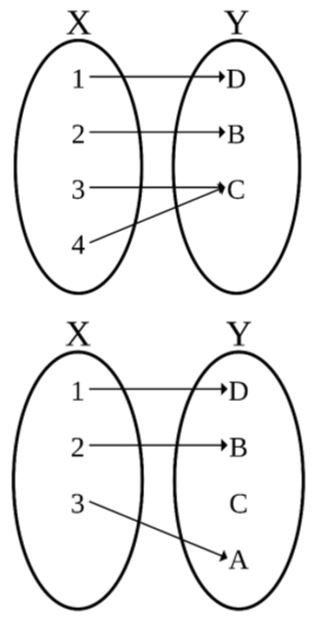
\includegraphics[width=2cm]{surj-inj.JPG}
			    \end{minipage}
			    \subsubsection{Bijektiv}
			        Jedes Element aus dem Wertebereich wird genau einmal getroffen\\ 
			        Bijektive Funktionen sind surjektiv und injektiv (es gilt:  \textbf{X = Y})\\
			        \vspace{-8pt}
			        \begin{itemize}
						\item $\forall y \in Y \exists ! x \in X: f(x)=y$
					\end{itemize}
					
			\subsection{Skalarprodukt}
					Ein inneres Produkt auf V ist eine Abbildung $\langle\bullet,\bullet\rangle: V\times V\rightarrow\mathbb{R}$ mit folgenden Eigenschaften:
					\begin{enumerate}
						\item Positive Definitheit: $\forall v\in V: \begin{cases}
						\langle v,v\rangle\ge0 \\
						\langle v,v\rangle=0\Leftrightarrow v=0\\
						\end{cases} $\\
						\item Bilinearität: 
						\begin{itemize}
							\item $\forall v,w,w'\in V:\langle v,w+w'\rangle=\langle v,w\rangle+\langle v,w'\rangle$
							\item $\forall v,w\in V, \alpha\in\mathbb{R}:\langle \alpha v,w\rangle=\alpha\langle v,w\rangle$
						\end{itemize}
						\item Symmetrie: $\forall v,w\in V:\langle v,w\rangle=\langle w,v\rangle$
					\end{enumerate}
					Diese Bedingungen gelten nur für $\mathbb{R}$-Vektorräume
					
		    \subsection{Normen}
					Eine Norm auf V ist eine Abbildung $\Vert\bullet\Vert:V\rightarrow\mathbb{R}$ mit:
					\begin{enumerate}
						\item Positive Definitheit:\\
						$\forall v\in V:\begin{cases}
						\Vert v\Vert\ge0 \\
						\Vert v\Vert=0\Leftrightarrow v=0\\
						\end{cases} $	
						\item Homogenität: $\forall v\in V,\alpha\in\C:\Vert\alpha v\Vert=\vert\alpha\vert\cdot\Vert v\Vert$
						\item Dreiecksungleichung: $\forall v,w\in V:\Vert v+w\Vert\le\Vert v\Vert+\Vert w\Vert$				
					\end{enumerate}
					\textbf{Äquivalenz der Normen}
					
					Jegliche zwei Normen $\Vert \cdot \Vert ^{(1)}$, $\Vert \cdot \Vert ^{(2)}$ sind äquivalent, d.h. $\exists C > 0$ s.d.
					
					$\frac{1}{C} \Vert x \Vert^{(1)} \leq \Vert x \Vert ^{(2)} \leq C \Vert x \Vert ^{(1)}, \ \forall x \in \R ^n$
					
					\textbf{Induzierte Normen}
					
					Man sagt, dass die Norm von einem Inneren Produkt induziert wird, wenn $\forall v\in V: \Vert v\Vert^2=\langle v,v\rangle$\\[4pt]
					\begin{example}
				 	    \textbf{Beispiele für Normen für $V=\mathbb{R}^n:$}
				 	    \begin{itemize}
				 		    \item Maximumnorm: $\Vert v\Vert_\infty=\max\{\abs{v_1},\abs{v_2},\dots,\abs{v_n}\}$
						    \item Euklid'sche Norm: $\Vert v\Vert_2=\sqrt{\abs{v_1}^2+\abs{v_2}^2+\dots+\abs{v_n}^2}$
						    \item p-Norm: $\Vert v\Vert_p=\big(\abs{v_1}^p+\abs{v_2}^p+\dots+\abs{v_n}^p)^{\frac{1}{p}},p\in\mathbb{N}$	
				 	    \end{itemize}
				 	    \textbf{Beispiele für Normen für $V=C^0(a,b):$}
					    \begin{itemize}
						    \item Maximumnorm: $\Vert f\Vert_\infty=\sup\abs{f(x)},\ x\in(a,b)$
						    \item Lp-Norm: $\Vert f\Vert_p=\Big(\int_a^b\abs{f(x)}^p\Big)^{\frac{1}{p}},p\in\mathbb{N}$
					    \end{itemize}
				    \end{example}
				\subsection{metrische Räume}
					Ein metrischer Raum (X,d) ist eine Menge X mit  einer Abstandsfkt.\\
					$d:X\times X\rightarrow\mathbb{R}$
					\begin{enumerate}
						\item Positive Definitheit: $\forall x,y:\ d(x,y)\ge0\ \& \ d(x,y)=0\Leftrightarrow x=y$
						\item Symmetrie: $\forall x,y\in X:\ d(x,y)=d(y,x)$
						\item Dreiecksungleichung: $\forall x,y,z\in X:\ d(x,z)\le d(x,y)+d(y,z)$
					\end{enumerate}
				\subsection{Vektoren}
					\textbf{(Euklidscher) Betrag}\\
					$ \vert x \vert = \Vert x \Vert = \sqrt{x_1^2 + \dots + x_n^2} \in \mathbb{R}^{\geqslant 0} $
					
					\textbf{Dreiecksungleichung}\\
					$ \vert x+y \vert \leqslant \vert x \vert + \vert y \vert $\\
					\textbf{(Euklidsches) Skalarprodukt}\\
					$ \langle x,y \rangle =  x_1 y_1 + \dots + x_n y_n \in \mathbb{R}^{n} $ f"ur zwei Vektoren $ x,y \in \mathbb{R}^{n} $\\
					\textbf{Kreuzprodukt}\\
					$   \vec{a}\times\vec{b}
  					=
  					\begin{pmatrix}a_1 \\ a_2 \\ a_3\end{pmatrix}
  					\times
  					\begin{pmatrix}b_1 \\ b_2 \\ b_3 \end{pmatrix}
  					=
  					\begin{pmatrix}
    					a_2b_3 - a_3b_2 \\
    					a_3b_1 - a_1b_3 \\
   					a_1b_2 - a_2b_1
  					\end{pmatrix}\ = |\vec{a}|\cdot|\vec{b}|\cdot \sin \alpha \cdot\hat{n}$ 
			
		\section{Folgen}
			\subsection{Konvergenzverhalten von Folgen}
		    	\subsubsection{Definition der Konvergenz}
			    Eine Folge $(a_n)_{n \in \N}$ konvergiert gegen a für $n \to \infty$, falls
			    
			    $\forall \epsilon > 0, \exists n_0 \in \N, \forall n \geq n_0: |a_n - a| < \epsilon$
			    
			    Man schreibt $\lim_{n\to\infty} a_n = a$, a ist der Grenzwert. Wenn der Limes existiert, dann ist die Folge $\textbf{konvergent}$, sonst ist sie $\textbf{divergent}$.
			    
			    \textbf{Nicht konvergieren} heisst nicht, dass eine Folge \textbf{divergiert}. Eine Folge kann weder konvergieren noch divergieren.
			    \subsubsection{Arten von Folgen}
			        \begin{itemize}
			            \item \textbf{Arithmetische Folge:} konstante Abstände zwischen Glieder, z.B. $\{1,2,3,4,...\}$
			            \item \textbf{Geometrische Folge:} konstante Verhältnisse zwischen Glieder, z.B. $\{2,4,8,16,32,...\}$
			            \item \textbf{Cauchy-Folge:} Abstände der Glieder werden beliebig klein, z.B. $\{1, \frac{1}{2}, \frac{1}{3}, \frac{1}{4}, \frac{1}{5}, ...\}$\\
			            \textbf{Jede konvergente Folge ist eine Cauchy-Folge!}
			            \item \textbf{Teilfolgen:} eine neue Folge, die entsteht, wenn Folgenglieder der ursprüng. Folge weggelassen werden, bspw. $b_n := a_{2n}$.\\
			            Ein \textbf{Häufungspunkt (HP)} einer Folge $a_n$ ist ein Punkt, der ein Grenzwert einer \textbf{unendlichen Teilfolge} von $a_n$ ist. Falls eine Folge mehrere HP hat, dann kann die Folge nie konvergieren. Der $\lim \sup_{n\rightarrow \infty}(a_n)$ berechnet den grössten HP.
			            \item \textbf{implizite Folgen:} von der Form $a_{n+1} = f(a_n)$. Falls die Folge beschränkt und monoton ist, dann existiert ein Grenzwert (Prop. aus VL). Somit muss man immer Monotonie und Beschränktheit beweisen (meist über Induktion). Grenzwerte sind i.d.R. schwierig zu berechnen, es gilt aber:\\ $\lim_{n \rightarrow \infty} f(a_n) = \lim_{n \rightarrow \infty} f(a_{n+1}) = a$
			        \end{itemize}
				\subsubsection{Wichtige Grenzwerte}
					\vspace{-10pt}
					\begin{align*}
						&\lim_{n\rightarrow \infty} \frac{1}{n^s}=0\hspace{10pt} \forall s\in \mathbb{Q^+} \hspace{5pt}\\
						&\lim_{n\rightarrow \infty} q^n=0 \hspace{10pt} \forall q\in \mathbb{C}\hspace{7pt} \vert q\vert <1\\					
						&\lim_{n\rightarrow \infty} \sqrt[n]{a}=1 \hspace{10pt} \forall a\in \mathbb{R^+} \hspace{5pt}\\
						&\lim_{n\rightarrow \infty} \frac{n^k}{z^n}=0 \hspace{10pt} \forall k \in \mathbb{N} \hspace{10pt} \forall z\in \mathbb{C} \hspace{10pt} \vert z\vert > 1\\						
						&\lim_{n\rightarrow \infty} \sqrt[n]{n}=1
					\end{align*}	
				\subsubsection{Berechnen von Grenzwerten}
				Der Limes ist ein linearer Operator und kommutiert mit Multiplikation/Division. $\lim_{n\to\infty} (\alpha a_n + \beta b_n) = \alpha \lim_{n\to\infty} (a_n) + \beta \lim_{n\to\infty} (b_n)$ und $\lim_{n\to\infty} (a_n \cdot b_n) = \lim_{n\to\infty} (a_n) \cdot \lim_{n\to\infty} (b_n)$
				\label{subsubsection:limitcalc}
					\begin{itemize}
						\item \textbf{Brüche:} Durch die grösste Potenz des Zählers/Nenners teilen
						\begin{example}
							\begin{equation*}
							\lim_{n\rightarrow \infty} \frac{4n^3+7n}{2n^3}=\lim_{n\rightarrow \infty} \frac{4+\frac{7}{n^2}}{2}=\frac{4}{2}=2
							\end{equation*}
						\end{example}						
						\item  \textbf{Wurzelterme:} Mit der 3. binomischen Formel erweitern
						\begin{example}
							\begin{align*}
							&\lim_{n\rightarrow \infty} n \left(\sqrt{1+\frac{1}{n}}-1\right) &\Vert \cdot \frac{\sqrt{1+\frac{1}{n}}+1}{\sqrt{1+\frac{1}{n}}+1}\\
							=&\lim_{n\rightarrow \infty} n\frac{1+\frac{1}{n}-1}{\sqrt{1+\frac{1}{n}}+1}\\
							=&\lim_{n\rightarrow \infty} \frac{\frac{n}{n}}{\sqrt{1+\frac{1}{n}}+1}=\frac{1}{\sqrt{1}+1}=\frac{1}{2}
							\end{align*}
						\end{example}						
						\item \textbf{Sonstige Terme:} Falls $a_n$ monoton (fallend/steigend) ist, dann suche eine untere Schranke $c_1(n) \le a_n \hspace{3pt} \forall n \in \mathbb{N}$ und eine obere Schranke $c_2(n) \ge a_n \hspace{3pt} \forall n \in \mathbb{N}$ mit $\lim\limits_{n \rightarrow \infty} c_1(n)=\lim\limits_{n \rightarrow \infty} c_2(n)=c$. Es gilt:
						$\lim\limits_{n \rightarrow \infty} a_n=c$
						\begin{example}
							\begin{align*}
								&a_n=\sqrt[n]{u^n+v^n} \hspace{10pt} u, v \in \mathbb{R}_{\ge 0} \hspace{10pt} u>v\\
								&\text{Untere Schranke: } a_n \ge \sqrt[n]{u^n}=u=c_1(n)\\
								&\text{Obere Schranke: } a_n \le \sqrt[n]{2u^n}=\sqrt[n]{2}u=c_2(n)\\
								&\lim_{n\rightarrow \infty}c_1(n)=\lim_{n\rightarrow \infty}c_2(n)=u \rightarrow \lim_{n\rightarrow \infty} a_n=u
							\end{align*}
						\end{example}					
					\end{itemize}
		\section{Reihen}
			\subsection{Geometrische Reihe}
				\begin{eq}
					\sum_{i=0}^{n}q^i= \frac{1-q^{n+1}}{1-q} \xrightarrow[n \to \infty]{} \frac{1}{1-q}\hspace{20pt} q \in \mathbb{C} \hspace{10pt} \vert q \vert <1
				\end{eq}
			\subsection{Allgemeine harmonische Reihe (Dirichlet-Reihe)}
				\begin{eq}
					\sum_{n=1}^{\infty} \frac{1}{n^s} \hspace{3pt}
					\begin{cases}							
						\text{konvergiert für} \hspace{5pt} &s>1\\
						\text{divergiert für} &s \le 1
					\end{cases}
				\end{eq}
			\subsection{Binomische Reihe}
				\begin{eq}
					(x+y)^{\alpha}=\sum_{k=0}^{\infty} \binom{\alpha}{k}x^{\alpha-k}y^k \hspace{15pt} \alpha \in \mathbb{C} \hspace{10pt} x, y \in \mathbb{R}
				\end{eq}
				\begin{example}
					\textbf{Anmerkungen}
					\begin{enumerate}
						\item[i)] Konvergenz, falls $x>0$ und $\left \vert \frac{y}{x}\right \vert <1$
						\item[ii)] Die Definition der allgemeinen Binomialkoeffizienten ist im Kapitel \ref{sec:binomial} auf Seite \pageref{sec:binomial}
					\end{enumerate}
				\end{example}	
			\subsection{Cauchy-Produktformel}
			Sind $\sum_{n=0}^{\infty}a_n$ und $	\sum_{n=0}^{\infty}b_n$	absolut konvergente Reihen, dann gilt
			\begin{equation*}
				\sum_{n=0}^{\infty}c_n=\left(\sum_{n=0}^{\infty}a_n\right)\cdot\left(\sum_{n=0}^{\infty}b_n\right)=\sum_{n=0}^{\infty}\sum_{k=0}^{n}a_kb_{n-k}
			\end{equation*}
			\subsection{Konvergenzkriterien}
				\subsubsection{Nullfolgenkriterium}
					Falls $a_n$ keine Nullfolge bildet, so divergiert die Reihe \[\sum_{n=0}^{\infty}a_n\]
				\subsubsection{Leibnitzkriterium}
					Falls $a_n$ eine monoton fallende Nullfolge bildet, dann konvergiert auch die alternierende Reihe \[\sum_{n=0}^{\infty} (-1)^n a_n\]
					\begin{annotation}{Zu zeigen:}
						\item[i)] $a_n \ge$ 0
						\item[ii)] $\lim_{n\rightarrow \infty} a_n$ =0
						\item[iii)] $a_{n+1} - a_n \le$ 0 oder $\frac{a_{n+1}}{a_n} \le 1$ (monoton fallend)
					\end{annotation}
					
					
				\subsubsection{Majorantenkriterium}
					Sei $\sum_{n=0}^{\infty}b_n$ eine konvergente Reihe und $a_n$ die Elemente einer Folge mit $a_n \le b_n \hspace{3pt} \forall n$, so konvergiert auch die Reihe $\sum_{n=0}^{\infty} a_n$
				\subsubsection{Minorantenkriterium}
					Sei $\sum_{n=0}^{\infty}b_n$ eine divergente Reihe und $a_n$ die Elemente einer Folge mit $a_n \ge b_n \hspace{3pt} \forall n$, so divergiert auch die Reihe $\sum_{n=0}^{\infty} a_n$ (meistens ist $\sum_{n=0}^{\infty}b_n$ die harmonische Reihe)\\\\
				    \begin{annotation}{Wann Major-, wann Minorantenkrit. verwenden:}
				        \item relative Ordnung der Reihe = (Grad Nenner) - (Grad Zähler)\\
				        \item Faustregel:
				        $\begin{cases}
				            \text{rel. Ordnung}>1 &\rightarrow \text{Majorantenkrit}\\
				            \text{rel. Ordnung}\leq1 &\rightarrow \text{Minorantenkrit}
				        \end{cases}$
				    \end{annotation}
				\subsubsection{Quotientenkriterium}
					\vspace{-10pt}
					\begin{equation*}
						Q=\lim_{n\rightarrow \infty} \left \vert\frac{a_{n+1}}{a_n}\right \vert \hspace{20pt} \sum_{n=0}^{\infty}a_n
						\begin{cases}
							\text{divergiert} \hspace{5pt} &Q>1\\
							\text{konvergiert absolut} &Q<1\\
							\text{keine Aussage} &Q=1
						\end{cases}
					\end{equation*}
				\subsubsection{Wurzelkriterium}
					\vspace{-10pt}
					\begin{equation*}
						L=\limsup_{n\rightarrow \infty} \sqrt[n]{\vert a_n \vert} \hspace{20pt} \sum_{n=0}^{\infty}a_n
						\begin{cases}
							\text{divergiert} \hspace{5pt} &L>1\\
							\text{konvergiert absolut} &L<1\\
							\text{keine Aussage} &L=1
						\end{cases}
					\end{equation*}
				\subsubsection{Integralkriterium}
					Sei $p \in \mathbb{Z}$, $f: [p, \infty) \rightarrow [0, \infty)$ monoton fallend und das Integral $\int_{p}^{\infty}f(x)$d$x$ existiert, dann konvergiert auch $\sum_{n=p}^{\infty}f(n)$ und es gilt die Abschätzung
					\begin{equation*}
						\sum_{n=p+1}^{\infty}f(n) \le \int_{p}^{\infty}f(x)\text{d}x \le \sum_{n=p}^{\infty}f(n)
					\end{equation*}	
				\subsubsection{Absolute Konvergenz}
				    Eine Reihe $\sum a_n$ konvergiert absolut, wenn $\sum \vert a_n \vert$ konvergiert. Absolute Konvergenz $\Rightarrow$ Konvergenz.
			\subsubsection{Normale Konvergenz (Funktionenreihe)}
			    Eine Funktionenreihe $\sum f_n$ konvergiert normal, falls $\exists b_n \forall n f_n(x) \leq b_n$ und die Reihe $\sum b_n$ konvergiert, wobei $b_n$ unabhängig von $x$ ist.  \\
			    \textit{Bem.: }$\exp, \sin$ konvergieren nicht normal auf ganz $\R$, da dies gleichm. Schranken über alle reellen Zahlen implizieren würde (aus MC).
			    
			\subsection{Potenzreihe}
				Eine Potenzreihe hat folgende Form
				\[f(x)=\sum_{n=1}^{\infty}a_n(x-x_0)^n \hspace{10pt} x_0: \text{Entwicklungspunkt}\]	
				\subsubsection{Wichtige Potenzreihen (Entwicklungspunkt P = 0)}
					\vspace{-7pt}
					\begin{align*}
						e^x&= \sum_{k=0}^{\infty}\frac{x^k}{k!}=1+x+\frac{x^2}{2!}+\frac{x^3}{3!}+\frac{x^4}{4!}+\cdots\\
						\cos(x)&=\sum_{k=0}^{\infty}(-1)^k \frac{x^{2k}}{(2k)!}=1-\frac{x^2}{2!}+\frac{x^4}{4!}-\frac{x^6}{6!}+\cdots\\
						\sin(x)&=\sum_{k=0}^{\infty}(-1)^k \frac{x^{2k+1}}{(2k+1)!}=x-\frac{x^3}{3!}+\frac{x^5}{5!}-\frac{x^7}{7!}+\cdots\\
						\arctan(x)&=\sum_{k=0}^{\infty}(-1)^k \frac{x^{2k+1}}{(2k+1)}=x-\frac{x^3}{3}+\frac{x^5}{5}-\frac{x^7}{7}+\cdots\\
						\cosh(x)&=\sum_{k=0}^{\infty} \frac{x^{2k}}{(2k)!}=1+\frac{x^2}{2!}+\frac{x^4}{4!}+\frac{x^6}{6!}+\cdots\\
						\sinh(x)&=\sum_{k=0}^{\infty} \frac{x^{2k+1}}{(2k+1)!}=x+\frac{x^3}{3!}+\frac{x^5}{5!}+\frac{x^7}{7!}+\cdots
					\end{align*}

					\begin{annotation}{Konvergenzradien  der Pozenzreihen}
					    \item für $e^x$, $cos(c)$, $sin(x)$, $cosh(x)$ und $sinh(x)$ ist der Konvergenzradius $\infty$, aufgrund der Fakultät im Nenner.
					    \item $\sum_{n=0}^\infty \frac{a^n}{n!}$ konvergiert absolut für alle $a\in\C$
					\end{annotation}
				\subsubsection{Konvergenzradius}
					Sei $R$ der Konvergenzradius einer Potenzreihe. Dann konvergiert die Potenzreihe absolut $\forall x \in \mathbb{C}$, $\vert x-x_0 \vert < R$ und divergiert für $\vert x-x_0 \vert > R$. Der Rand $|x - x_0 | = R$ muss separat betrachtet werden. \\
					\textbf{Berechnungsarten: }
					\setlength{\columnseprule}{0pt}
					\begin{multicols}{2}
						\begin{itemize}
						\item $R = \lim_{n\to\infty} \left\vert \frac{a_n}{a_{n+1}}\right\vert$
					    \item $R = \frac{1}{\lim_{n\to\infty} \sqrt[n]{\vert a_n \vert}}$
						\end{itemize}
					\end{multicols}
					\setlength{\columnseprule}{0.5pt}
		\section{Funktionen}
			\subsection{Berechnen von Grenzwerten}
			    \subsubsection{Dominanzen}
			        Die Sachen die links stehen wachsen langsamer als die Sachen die rechts stehen:\\
			        $\log{(n)}\prec\log^2{(n)}\prec\dots\prec\ n^{\frac{1}{3}}\prec\sqrt{n}\prec n\prec n^2\prec\dots\prec e^n\prec n!\prec n^n$
				\subsubsection{Brüche}
					Durch die grösste/kleinste Potenz des Zählers/Nenners teilen
				\subsubsection{Beträge}
					Beträge vereinfachen indem man sich überlegt, ob das Argument im Betrag grösser bzw. kleiner 0 ist\\\\
					\begin{example}
						\textbf{Beispiel}
						\begin{equation*}
							\lim_{x \rightarrow 2^-} \frac{4-x^2}{\vert x-2 \vert} = \lim_{x \rightarrow 2^-} \frac{4-x^2}{2-x} = \lim_{x \rightarrow 2^-} (2+x) = 4
						\end{equation*}
					\end{example}
				\subsubsection{Wurzelterme}
					Wurzelterme kann man meistens mithilfe der 3. binomischen Formel erweitern\\\\
					\begin{example}
						\textbf{Beispiel}
						\begin{equation*}
							\lim_{x \rightarrow \infty} \sqrt{x^2+x}-x = \lim_{x \rightarrow \infty} \frac{x^2+x-x^2}{\sqrt{x^2+x}+x} = \lim_{x \rightarrow \infty} \frac{1}{\sqrt{1+\frac{1}{x}}+1}=\frac{1}{2}
						\end{equation*}
					\end{example}
				\subsubsection{Beschränktheit einer Funktion}
					Man kann die Beschränktheit einer Funktion (v.a. trig. Fkt.) ausnutzen um Grenzwerte zu berechnen\\\\
					\begin{example}
						\textbf{Beispiel}
						\begin{equation*}
							\lim_{x \rightarrow 0} x^2 \sin \left(\frac{1}{x} \right) = 0
						\end{equation*}
					\end{example}
				\subsubsection{Sandwich-Theorem}
					Seien $(x_n),(y_n),(z_n)$ Folgen so dass $x_n\le y_n\le z_n$\\ mit $\lim_{n \rightarrow \infty} x_n= \lim_{n \rightarrow \infty} z_n=c$, dann muss auch $\lim_{n \rightarrow \infty} y_n=c $ \\\\
					\begin{example}
						\textbf{Beispiel} siehe \ref{subsubsection:limitcalc} ''Sonstige Terme'' \end{example}
				\subsubsection{Potenzreihen}
					Falls die Potenzreihe der Funktion bekannt ist, kann man sie durch die Potenzreihe darstellen
				\subsubsection{l'Hospitalsche Regel (bei Folgen nicht verwendbar!)}
				Für $\frac{0}{0}, \frac{\infty}{\infty}, 0\cdot\infty, 0^0, \infty^0, 1^\infty, \infty - \infty$ Mögliche Umformungen: $f\cdot g = \frac{f}{1/g}$ oder $f-g = \frac{1}{1/f}-\frac{1}{1/g} = \frac{1/g - 1/f}{1/(f\cdot g)}$
					\begin{eq}
						\lim_{x \rightarrow x_0} \frac{f(x)}{g(x)}=\lim_{x \rightarrow x_0} \frac{f'(x)}{g'(x)}= \cdots =\lim_{x \rightarrow x_0} \frac{f^{(n)}(x)}{g^{(n)}(x)}
					\end{eq}
				\subsubsection{''exp-log'' Methode}
					\begin{eq}
						\lim_{x \rightarrow x_0} g(x)^{h(x)}=\exp\left(\lim_{x \rightarrow x_0} h(x) \cdot \ln(g(x))\right)
					\end{eq}
					\begin{example}
						\textbf{Beispiel}
						\begin{align*}
							\lim_{x \rightarrow 0}(1+3\sin(x))^{\frac{1}{x}}&=\exp \left(\lim_{x \rightarrow 0} \frac{\ln(1+3\sin(x))}{x}\right)\\
							&=\exp \left(\lim_{x \rightarrow 0} \frac{3 \cos(x)}{1+3\sin(x)}\right)\\
							&=e^3
						\end{align*}
					\end{example}
					\begin{example}
						\textbf{Trick}
						\begin{align*}
        				     \exp(\lim_{x \rightarrow 0}\ln (x) \cdot x) &=\exp(\lim_{x \rightarrow 0} \frac{\ln (x)}{\frac{1}{x}})\\  
        				     &(= \exp(\lim_{x \rightarrow 0} \frac{\frac{1}{x}}{\frac{-1}{x^2}}) = e^0 = 1)
						\end{align*}
					\end{example}
				\subsubsection{Substitution}
					\begin{equation*}
						\lim_{x \rightarrow x_0} f(x)=\lim_{u \rightarrow u_0} f(u) \hspace{10pt} \text{mit } u_0=\lim_{x \rightarrow x_0} u(x)\\
					\end{equation*}
					\begin{example}
						\textbf{Beispiel}
						\begin{align*}
							&\lim_{x \rightarrow 0^+} x\ln(x) \hspace{25pt} u(x)=-\ln(x) \rightarrow x=e^{-u}\\
							&u_0=\lim_{x \rightarrow 0^+} -\ln(x)=\infty\\
							&\lim_{x \rightarrow 0^+} x\ln(x)=\lim_{u \rightarrow \infty} -ue^{-u}=0
						\end{align*}
					\end{example}
			\subsection{Stetigkeit}
				\subsubsection{Epsilon-Delta-Kriterium}
				\begin{equation*}
					\forall \varepsilon > 0, \hspace{2pt} \exists \delta > 0, \hspace{2pt} \forall x \in \mathbb{R}: \vert x-x_0 \vert < \delta \implies \left \vert f(x)-f(x_0) \right \vert < \varepsilon
				\end{equation*}
				\\
				Wie finde ich zu jedem $\varepsilon > 0$ das passende  $\delta$?
				\begin{enumerate}
						\item Beginne mit $\left \vert f(x)-f(x_0) \right \vert < \varepsilon$ und finde einen Ausdruck so dass:
				        $\left \vert f(x)-f(x_0) \right \vert \le ...\vert x-x_0 \vert ... < \varepsilon$
						\item Setze ein: $\vert x-x_0 \vert < \delta$
						\item $\left \vert f(x)-f(x_0) \right \vert \le ...\vert x-x_0 \vert ... <  ...\delta... <\varepsilon$
						\item Benutze $...\delta... <\varepsilon$ um $\delta(x_0, \varepsilon)$ zu finden
						\item Zeige, dass wirklich $\vert x-x_0 \vert < \delta \implies \left \vert f(x)-f(x_0) \right \vert < \varepsilon$
					\end{enumerate}
				
				\subsubsection{Grenzwert-Kriterium}
					\begin{equation*}
						\lim_{x \rightarrow x_0} f(x) \overset{!}{=} f(x_0) 
					\end{equation*}
					\begin{annotation}{Anmerkung}
						\item[i)] Wenn nichts anderes verlangt wird, wird die Stetigkeit meistens mit dem Grenzwert-Kriterium gezeigt
						\item[ii)] \textbf{Achtung:} Bei einem $x_0 \neq \infty$ oder $x_0 \neq-\infty$ muss der Grenzwert von beiden Seiten berücksichtigt werden!
					\end{annotation}
				\subsubsection{Stetige Funktionen}
					\setlength{\columnseprule}{0pt}
					\begin{multicols}{2}
						\begin{itemize}
							\item Polynome
							\item rationale Funktionen (Nenner $\ne 0$)
							\item trig. Funktionen
							\item hyperbolische Funktionen
							\item Exponentialfunktion
							\item Logarithmusfunktion
							\item Komposition von stetigen Funktionen
						\end{itemize}
					\end{multicols}
					\setlength{\columnseprule}{0.5pt}
				\subsubsection{Lipschitz Stetigkeit}
					\begin{eq}
						\left \vert f(x)-f(y) \right \vert \le  L \vert x-y \vert \hspace{15pt} L\ge 0 \hspace{15pt} \forall x, y \in \mathbb{R}\\
					\end{eq}
					\begin{annotation}{Anmerkung}
						\item[i)] Lipschitz-stetige Funktionen sind insbesondere stetig
						\item[ii)] Falls $f$ diffbar, dann: $L = \underset{x}{\max} |f'(x)|$
					\end{annotation}
					\begin{example}
		                \textbf{Beispiel. } $f(x) = x^2$ ist Lipschitz-stetig auf $[0,1]$, weil $L = \underset{x}{\max} |f'(x)| = 2$, aber $f$ ist \underline{nicht} Lip.-stetig auf $\R$, weil $L = \underset{x}{\max} |f'(x)| = |2x| = \infty$
					\end{example} 
			    \subsubsection{topologische Stetigkeit}
			        Falls für jede offene Teilmenge $U \subset Y$ das Urbild $f^{-1}(U)$ offen in $X$ ist, dann heisst die Funktion topologisch stetig.
				\subsubsection{Stetigkeit überprüfen (1-dim)}
					\begin{align*}
						&f(x)=
						\begin{cases}
							f_1(x) \hspace{10pt} &x<p\\
							f_2(x) & x>p\\
							a &x=p\\							
						\end{cases}
						&\lim_{x \rightarrow p^-} f_1(x) \overset{!}{=} \lim_{x \rightarrow p^+} f_2(x) \overset{!}{=} a
					\end{align*}
				\subsubsection{Stetigkeit überprüfen (n-dim)}
					Der Limes $\lim\limits_{x \rightarrow x_0} f(x) \hspace{5pt} x \in \mathbb{R}^n$ muss existieren und eindeutig sein.\\ Im $\R^2$ den Polarkoordinatentrick nutzen, um jede Richtung auf einmal betrachten zu können ($x \mapsto r\cos(\theta), y \mapsto r\sin(\theta)$). \\
					\begin{annotation}{Anmerkungen}
						\item [i)] Falls $n=2$: Transformiere $x$ und $y$ in Polarkoordinaten, $\varphi$ muss sich dabei rauskürzen, da der Limes sonst nicht eindeutig ist
						\item [ii)] Falls $n>2$: Nur zeigen, dass der Grenzwert nicht eindeutig ist, sonst zu kompliziert
					\end{annotation}
			\subsection{Punktweise und gleichmässige Konvergenz}
			    \subsubsection{Punktweise Konvergenz}
			        Eine Funktionenfolge $f_n$ konvergiert punktweise gegen ihre Grenzfunktion $f$, wenn für jedes $x$ im Definitionsbereich gilt: $f_n(x) \rightarrow f(x)$. Die Grenzfunktion $f$ muss dabei \textit{nicht} stetig sein. \\\\
					\begin{example}
						\textbf{Beispiel}
						\begin{equation*}
							f_n : [0,1] \rightarrow \R : \hspace{5pt} f_n(x) = x^n 
						 \end{equation*}
						 \begin{equation*}
						    \lim_{n\rightarrow \infty}f_n = f = 
							\begin{cases}
    							1, \hspace{5pt} &x=1\\
    							0, & x<1
    						\end{cases}
						\end{equation*}
					\end{example}
				\subsubsection{Gleichmässige Konvergenz}
				    Eine Funktionenfolge $f_n$ konvergiert gleichmässig gegen ihre Grenzfunktion $f$, falls gilt
				    \begin{equation*}
				        \vert f(x)-f_n(x) \vert \leq b_n
				    \end{equation*}
				    wobei die Folge $b_n$ unabhängig von $x$ ist und gegen $0$ konvergiert. Sind die Folgenglieder $f_n$ stetig, ist in diesem Fall auch die Grenzfunktion $f$ stetig.  \\
				    Gleichmässige Konv. ($\exists\epsilon\forall x$) $\Rightarrow$ Punktweise Konv. ($\forall x \exists\epsilon$)
				    
		\section{Differentialrechnung}
			\subsection{Eindimensionale Differentialrechnung}
				Eine Funktion heisst differenzierbar, falls der Grenzwert
				\begin{equation*}
					\lim_{x\rightarrow x_0} \frac{f(x)-f(x_0)}{x-x_0}=\lim_{h \rightarrow 0} \frac{f(x_0+h)-f(x_0)}{h}
				\end{equation*}
				existiert (und somit eindeutig ist) $\rightarrow$ punktweise Eigenschaft
				\subsubsection{Regeln}
					\begin{itemize}
						\item \textbf{Produktregel} \[(f \cdot h)'=f'(x) \cdot g(x)+f(x) \cdot g'(x)\]
						\item \textbf{Quotientenregel} \[\left(\frac{f}{g}\right)'=\frac{f'(x) \cdot g(x)-f(x) \cdot g'(x)}{g(x)^2}\]
						\item \textbf{Kettenregel}
						\[\left(f \circ g\right)'(x)= f'(g(x)) \cdot g'(x)\]
						(Trick: $a^x = e^{x \ln (a)}= e^{\ln(a^x)}$)
						\item \textbf{Umkehrregel}
						\[\left(f^{-1}\right)'(y)=\frac{1}{f'\left(f^{-1}(y) \right)}\]
						\item \textbf{Potenzregel}
						\[\left(x^n\right)' = n \cdot x^{n-1}\]
						\item \textbf{Log. Ableitung}
						\[\left( \ln(f)\right)' = \frac{f'(x)}{f(x)}\]
					\end{itemize}
				\subsubsection{Entwicklung}
					\begin{itemize}
						\item \textbf{Taylorpolynom}
						\begin{equation*}
							T_Nf(x; x_0)=\sum_{k=0}^{N}\frac{f^{(k)}(x_0)}{k!}(x-x_0)^k
						\end{equation*}
						\item \textbf{Fehlerabschätzung}
						\begin{equation*}
							R_N(x;x_0)=\frac{f^{(N+1)}(\xi)}{(N+1)!}(x-x_0)^{N+1} \hspace{20pt} \xi \in [x_0, x]
						\end{equation*}
						\item \textbf{Taylorreihe}
						\begin{equation*}
							Tf(x, x_0)=\sum_{k=0}^{\infty} \frac{f^{(k)}(x_0)}{k!}(x-x_0)^k
						\end{equation*}
					\end{itemize}
					\begin{annotation}{Anmerkung}
						\item[i)] Falls die Taylorreihe mit der Potenzreihe übereinstimmt, nennt man die Funktion analytisch und es gilt $Tf(x, x_0)=f(x)$
					\end{annotation}
					\textbf{Konvexität: } $f''(x) \geq 0$ (siehe auch \ref{sec:konvex}, Seite \pageref{sec:konvex})
			\subsection{Mehrdimensionale Differentialrechnung}	
				\subsubsection{Richtungsableitung}
					\begin{equation*}
						D_vf(\textbf{x})=\lim_{h \rightarrow 0}\frac{f(\textbf{x}+h \cdot \textbf{v})-f(\textbf{x})}{h} \hspace{10pt} \textbf{v} \in \mathbb{R}^n
					\end{equation*}	
					Partielle Ableitung: Achsenrichtungen $x_1, \dots, x_n$ einsetzen. \\
					
					Die Richtungsableitung kann auch mithilfe des Gradienten berechnet werden. Es gilt:
					\begin{itemize}
						\item $\partial_ef(x_0)=\vec{e}\cdot\nabla f(x_0)$ \hspace{10pt} wobei $\vec{e}$ normiert ist (Länge 1)
					\end{itemize}
					
				\subsubsection{Differenzierbarkeit}
					Sei $U \in \mathbb{R}^n$ eine offene Menge, $\textbf{x}, \textbf{x}_0 \in U$ Vektoren und $Jf(\textbf{x})$ eine lineare Abbildung. Die Funktion (Skalarfeld) $f: U \rightarrow \mathbb{R}$ ist (total) differenzierbar in $\textbf{x}_0$, falls der folgende Grenzwert existiert und eindeutig ist
			
					\begin{align*}
						0 &\overset{!}{=} \lim_{\textbf{x} \rightarrow \textbf{x}_0} \frac{f(\textbf{x})-f(\textbf{x}_0)-Jf(\textbf{x}_0) \cdot (\textbf{x}-\textbf{x}_0)}{\vert \vert \textbf{x}-\textbf{x}_0 \vert \vert}\\
						&= \lim_{\textbf{h} \rightarrow 0} \frac{f(\textbf{x}_0+\textbf{h})-f(\textbf{x}_0)-Jf(\textbf{x}_0)\cdot \textbf{h}}{\vert \vert \textbf{h} \vert \vert} 
					\end{align*}
			
					\begin{annotation}{Anmerkungen}
						\item[i)] $Jf(\textbf{x})$ entspricht der Jacobi-Matrix, also der ersten totalen Ableitung bezüglich der Standartbasen von $\mathbb{R}^n$ (und $\mathbb{R}^m$ für Vektorfelder)
						\item[ii)] $\textbf{h}$ kann man sich als kleine Änderung vorstellen (im Grenzwert wird $\textbf{h}$ ein Differential)
						\item[iii)] Die Funktion ist (total) differenzierbar, falls sie in jedem Punkt ihres Definitionsbereiches (total) differenzierbar ist
						\item[iv)] Meistens schreibt man nur differenzierbar und meint damit totale 
						\item[v)] Alle partiellen Ableitungen von $f$ existieren und sind stetig in $x_0 \Rightarrow$ die totale Abletiung $\d f(x_0) = (\frac{\partial f}{x_1}, \cdots, \frac{\partial f}{x_n})$ existiert. (Achtung: $\not\Leftarrow$)
					\end{annotation}
				\subsubsection{Vorgehen um Differenzierbarkeit zu zeigen}
					Funktionen die aus diffbaren Funktionen besteht, darf man als diffbar annehmen, somit muss man meistens nur einen Punkt $\textbf{x}_0$ auf (totale) Differenzierbarkeit überprüfen
					\begin{enumerate}
						\item Partielle Ableitungen über die Definition im Punkt $\textbf{x}_0$ berechnen. Falls die partiellen Ableitungen nicht existieren, dann ist die Funktion nicht (total) differenzierbar
						\item Falls die partiellen Ableitungen stetig sind, dann ist auch die Funktion (total) differenzierbar
						\item Die lineare Abbildung $Jf(\textbf{x}_0)$ im Punkt $\textbf{x}_0$ berechnen
						\item $Jf(\textbf{x}_0)$ in die Definition einsetzen und Grenzwert berechnen. Die Funktion ist (total) differenzierbar in $\textbf{x}_0$, falls die Definition erfüllt ist
					\end{enumerate}
				\subsubsection{Gradient}
				    \label{sec:Gradient}
					\vspace{-5pt}
					\begin{equation*}
						\nabla f(x)=
						\begin{pmatrix}
							\frac{\partial f(x)}{\partial x_1}\\
							\vdots\\
							\frac{\partial f(x)}{\partial x_n}
						\end{pmatrix} (=df(x))
					\end{equation*}
				\subsubsection{Jacobi-Matrix (Funktionalmatrix)}
					\begin{equation*}
						J_f(x) = \d f (x) = 
						\begin{pmatrix}
							\frac{\partial f_1(x)}{\partial x_1} &\cdots &\frac{\partial f_1(x)}{\partial x_n}\\
							\vdots &\ddots &\vdots\\
							\frac{\partial f_m(x)}{\partial x_1 } &\cdots &\frac{\partial f_m(x)}{\partial x_n}
						\end{pmatrix}
					\end{equation*}
				\subsubsection{Hesse-Matrix (für Skalarfelder)} 
					\begin{equation*}
						H_f(x)=
						\begin{pmatrix}
							\frac{\partial^2f(x)}{\partial x_1^2} &\cdots &\frac{\partial^2f(x)}{\partial x_1 \partial x_n}\\
							\vdots &\ddots &\vdots\\
							\frac{\partial^2f(x)}{\partial x_n \partial x_1} &\cdots &\frac{\partial^2f(x)}{\partial x_n^2}
						\end{pmatrix} \hspace{6pt}  \text{\small(symmetrisch!)}
					\end{equation*}
				\subsubsection{Implizite Differentiation}
					Erfüllt die Funktion $f:\mathbb{R} \rightarrow \mathbb{R}$ die Gleichung $F(x, f(x))=0$ und gilt $F_y(x_0, y(x_0)) \ne 0$, dann ist die Ableitung von $f$ gegeben durch
					\[f'(x)=-\frac{F_x(x, f(x))}{F_y(x, f(x))}\]
					\begin{example}
						\textbf{Beispiel}
						\begin{align*}
							&F(x, y)=x-2y^3-3y^5-y=0\\
							&\frac{\partial F}{\partial x}=1 \hspace{20pt} \frac{\partial F}{\partial y}=-6y^2-15y^4-1\\
							&\rightarrow y'(x)=\frac{1}{6y^2+15y^4+1}
						\end{align*}
					\end{example}
					\begin{annotation}{Anmerkung}
						\item[i)] Falls $f$ mehrdimensional ist, dann wende das implizite Funktionentheorem an (Kapitel \ref{sec:impl} Seite \pageref{sec:impl}) 
					\end{annotation}
				\subsubsection{Allgemeine Kettenregel}
					Seien $\textbf{f}:\mathbb{R}^n \rightarrow \mathbb{R}^L$ und $\textbf{g}:\mathbb{R}^L \rightarrow \mathbb{R}^m$ differenzierbare Funktionen, dann ist die Ableitung von $\textbf{h}:\mathbb{R}^n \rightarrow \mathbb{R}^m, \* \textbf{h}=\textbf{g} \circ \textbf{f}$ im Punkt $\textbf{p} \in \mathbb{R}^n$ gegeben durch
					\begin{align*}
						&D(\textbf{g}\circ \textbf{f})_{\textbf{p}} =D\textbf{g}_{\textbf{f}(\textbf{p})}\cdot D\textbf{f}_{\textbf{p}}\\
						&J_{\textbf{g}\circ \textbf{f}}(\textbf{p}) =J_{\textbf{g}}(\textbf{f}(\textbf{p}))\cdot J_{\textbf{f}}(\textbf{p})
					\end{align*}
				\subsubsection{Taylorentwicklung}
					\begin{itemize}
						\item \textbf{Taylorpolynom 2-ter Ordung}
						\begin{equation*}
							T_{2}f(x, a)=f(a)+\nabla f(a)^T(x-a)+\frac{1}{2}(x-a)^TH_f(a)(x-a)
						\end{equation*}
						\item \textbf{Taylorpolynom 3-ter Ordung}
						\begin{align*}
							T_{3}f(x, a)&=f(a)+ \triangle x_1 \partial_{x_1}f(a) + \triangle x_2 \partial_{x_2} f(a)\\
							&+ \frac{1}{2}(\triangle x_1)^2 \partial_{x_1 x_1} f(a) + \triangle x_1\triangle x_2 \partial_{x_1 x_2} f(a) \\
							&+ \frac{1}{2}(\triangle x_2)^2 \partial_{x_2 x_2} f(a)+ \frac{1}{6}(\triangle x_1)^3 \partial_{x_1 x_1 x_1} f(a)\\
							&+ \frac{1}{2} (\triangle x_1)^2 \triangle x_2 \partial_{x_1 x_1 x_2} f(a)\\
							&+ \frac{1}{2} \triangle x_1 (\triangle x_2)^2 \partial_{x_1 x_2 x_2} f(a)\\
							&+ \frac{1}{6}(\triangle x_2)^3 \partial_{x_2 x_2 x_2} f(a)
						\end{align*}
						\item \textbf{Taylorpolynom n-ter Ordnung}
							\begin{equation*}
								T_nf(x, a)=\sum_{k=0}^{n} \frac{1}{k!}\left(\Delta x_1 \frac{\partial}{\partial x_1}+\cdots+\Delta x_n \frac{\partial}{\partial x_n}\right)^kf(x)\Bigg|_{x=a}
							\end{equation*}
					\end{itemize}
					\begin{annotation}{Anmerkungen}
						\item [i)] $\Delta x_i$ bezeichnet die Differenz $(x_i-a_i)$
						\item [ii)] Es wird zuerst die Funktion partiell abgeleitet und erst danach am Punkt $a$ ausgewertet
						\item [iii)] Die Tangentialebene ist das Taylorpolynom erster Ordnung 
					\end{annotation}
					
				\subsubsection{Zusammenhänge \& Implikationen}
				\begin{itemize}
				    \item $f$ stetig differenzierbar $\Longrightarrow f$ differenzierbar $\Longrightarrow f$ partiell differenzierbar $\Longrightarrow f$ stetig 
				    \item $f$ partiell diff'bar in $x_0$ + part. Abl. stetig an Stelle $x_0$ $\Longrightarrow f$ diff'bar in $x_0$ 
				    \item $f$ partiell diff'bar in $x_0$ + part. Abl. stetig in Umgebung von $x_0$ $\Longrightarrow f$ stetig diff'bar in $x_0$
				\end{itemize}
				
			\subsection{Extremwerte ohne Nebenbedingungen}
				\subsubsection{Eindimensionale Funktion}
					\begin{enumerate}
						\item \textbf{Kandidaten}
							\begin{itemize}
								\item Intervallgrenzen (globale Extrema)
								\item $f'(x) \overset{!}{=}0$
							\end{itemize}
						\item \textbf{Art von Extrema}
							\begin{itemize}
								\item (lokales) Maximum: $f''(x_0)<0$
								\item (lokales) Minimum: $f''(x_0)>0$
							\end{itemize}
						\item \textbf{Vergleich lokale und globale Extrema}
					\end{enumerate}
				\subsubsection{Mehrdimensionale Funktion}
					\begin{enumerate}
						\item \textbf{Kandidaten}
						\begin{equation*}
							\nabla f(x_0)\overset{!}{=}0
						\end{equation*}
						\item \textbf{Art von Extrema}
							\begin{itemize}
								\item $H_f(x_0)$ negativ definit $\Rightarrow Maximum$
								\item $H_f(x_0)$ positiv definit $\Rightarrow Minimum$
								\item $H_f(x_0)$ indefinit $\Rightarrow Sattelpunkt$
								\item $H_f(x_0)$ semidefinit $\Rightarrow unbekannt$
								\item$\not \Leftarrow$: es könnte auch semidefinit sein.
							\end{itemize}
							
						\vspace{8pt}
						F"ur eine symmetrische reelle \(2\times2\)-Matrix
						\vspace{-4pt}
						\begin{equation*}
						    A =
						    \begin{pmatrix}
							    a&b\\c&d
						    \end{pmatrix}
						    \hspace{3pt}  \text{und} \hspace{3pt}\det(A) = a\cdot d - b\cdot c \hspace{3pt} \text{gilt:}
					    \end{equation*}
					    \vspace{-15pt}
						
					    \begin{itemize}
						    \item	\emph{positiv definit} \(\Longleftrightarrow\) \(a>0\) und \(\text{det}(A)>0\)
						    \item	\emph{negativ definit} \(\Longleftrightarrow\) \(a<0\) und \(\text{det}(A)>0\)
						    \item	\emph{indefinit} \(\Longleftrightarrow\) \(\text{det}(A)<0\) (Sattelpunkt)
						    \item	\emph{semidefinit}     \(\Longleftrightarrow\)     \(\text{det}(A)=0\)
						    \item   $0$\emph{-Matrix} ist pos/neg \underline{semi}-definit $\Rightarrow$ keine Aussage möglich
					    \end{itemize}
					\end{enumerate}
					\begin{annotation}{Anmerkungen}
						\item[i)] Definitheit von Matrizen Kapitel \ref{sec:definitheit} (Seite \pageref{sec:definitheit})
						\item[ii)] Falls $H_f(x_0)$ semipositiv bzw. seminegativ definit ist, kann keine Aussage zur Art des Extremums getroffen werden
						\item[iii)] Wenn $H_f(x)$ negativ definit (positiv definit) ist, dann ist $f$ konkav (konvex)
					\end{annotation}
			\subsection{Extremwerte mit Nebenbedingungen}
				\begin{align*}
					&\nabla L(\textbf{x}_0) \overset{!}{=} \textbf{0} \hspace{30pt} \text{mit } L=f(\textbf{x})-\sum_{i=1}^{n}\lambda_i \varphi_i\\
					&\varphi_i :\text{Nebenbedingungen} \hspace{15pt} \lambda_i: \text{Lagrange-Multiplikatoren}
				\end{align*}
				\subsubsection{Vorgehen}
					\begin{enumerate}
						\item Nebenbedingungen zeichnen
						\item Menge sollte abgeschlossen und beschränkt sein $\rightarrow$ existiert ein Maximum/Minimum (wegen Extremumsatz) (die Funktion sollte natürlich auf dem Bereich auch stetig sein)
						\item Gradienten berechnen
						\begin{itemize}
							\item[i)] innere Punkte: $\nabla f(\textbf{x}_0)\overset{!}{=} \textbf{0}$ ($\textbf{x}_0$ muss Element der Menge sein)
							\item[ii)] Randpunkte: $\nabla L\overset{!}{=} \textbf{0}$ 
						\end{itemize}
						\item Löse Gleichungssystem mit Nebenbedingungen
						\item Kandidaten der Extrema + Eckpunkte ($\nexists$ Ableitung) aufschreiben
						\item Kandidaten in $f(\textbf{x})$ einsetzen und vergleichen
					\end{enumerate}
					\begin{example}
						\textbf{Beispiel}
						\begin{equation*}
							f(x, y, z)=4y-2z \hspace{15pt} \varphi_1=x^2+y^2-1 \hspace{10pt} \varphi_2=2x-y-z-2
						\end{equation*}
						\begin{enumerate}
							\item Nebenbedingungen zeichnen
							\item $f(x, y, z)$ ist stetig und die Menge M ist beschränkt und abgeschlossen $\rightarrow \exists$ Max/Min
							\item keine inneren Punkte (schräg im Raum liegende Ellipse)
							\begin{equation*}
								\nabla \varphi_1=
								\begin{pmatrix}
									2x\\ 2y\\ 0
								\end{pmatrix}
								\hspace{10pt} \nabla \varphi_2=
								\begin{pmatrix}
									2\\ -1\\-1
								\end{pmatrix}
								\hspace{10pt} \nabla f=
								\begin{pmatrix}
									0\\ 4\\ -2
								\end{pmatrix}
							\end{equation*}
							\item Gleichungssystem lösen \hspace{10pt} $\nabla f=\lambda_1 \nabla \varphi_1+\lambda_2 \nabla \varphi_2$
							\begin{multicols*}{2}
								\begin{itemize}
									\item[I: ] $0 =2 \lambda_1 x+2 \lambda_2$
									\item[II: ] $4=2 \lambda_1 y-\lambda_2$
									\item[III: ] $2=\lambda_2$
									\item[IV: ] $1=x^2+y^2$
									\item[V: ] $2=2x-y-z$
								\end{itemize}
							\end{multicols*}
							\begin{tabular}{ccc}
								$\lambda_1=\pm \sqrt{13}$ &$\lambda_2 =2$ &$x=\mp \frac{2}{\sqrt{13}}$\\
								$y=\pm \frac{3}{\sqrt{13}}$ &$z=\mp \frac{7}{\sqrt{13}-2}$ &\\
							\end{tabular}
							\item Punkte aufschreiben
							\begin{align*}
								P_1&=\left(\frac{-2}{\sqrt{13}}, \frac{3}{\sqrt{13}}, \frac{-7}{\sqrt{13}}-2 \right)\\
								P_2&=\left(\frac{2}{\sqrt{13}}, \frac{-3}{\sqrt{13}}, \frac{7}{\sqrt{13}}-2 \right)\\
							\end{align*}
							\item Punkte vergleichen
							\begin{align*}
								f(P_1)&=\frac{26}{\sqrt{13}}+4\\
								f(P_2)&=\frac{-26}{\sqrt{13}}+4
							\end{align*}
							Somit ist $P_1$ ein Maximum und $P_2$ ein Minimum
						\end{enumerate}
					\end{example}
					\begin{annotation}{Anmerkungen}
						\item[i)] Es kann sein, dass der Rand nicht durch Nebenbedingungen darstellbar ist, dann kann man die Funktion direkt für den Rand auswerten und die Funktionswerte vergleichen
						\item[ii)] Man kann den Rand auch parametrisieren und die Parametrisierung in $f(\textbf{x})$ einsetzen. Jetzt kann man wie gewohnt die Ableitung gleich 0 setzen und die Kandidaten berechnen vergleichen\\
						Randpunkte nicht vergessen
					\end{annotation}
		\section{Gewöhnliche Differentialgleichungen (ODE)}
			\subsection{Separierbare Differentialgleichung}
				Falls eine DGL folgende Form hat, dann gilt
				\begin{equation*}
					y'=p(y)q(x) \rightarrow \int \frac{1}{p(y)} \text{d}y=\int q(x) \text{d}x
				\end{equation*}
				Wenn man die Integrale löst, erhält man eine implizite Gleichung. $y$ explizit darzustellen kann schwierig sein, zumal man die Lösungsmenge nicht verändern darf\\\\
				\begin{example}
					\textbf{Beispiel}
					\begin{align*}
						yy' + 2=0 \rightarrow \int y \text{d}y&=\int -2 \text{d}x\\		
						\frac{y^2}{2}&=-2x + C_1 \hspace{10pt} C_1 \in \mathbb{R}\\
						y&=\pm \sqrt{-4x + C_2}				 
					\end{align*}
				\end{example}
			\subsection{Lineare Differentialgleichung}
				Eine lineare DGL der n-ten Ordnung hat folgende Form
				\begin{equation*}
					a_0y^{(0)}+\dots+ a_ny^{(n)}=q(x)
				\end{equation*}
				\begin{annotation}{Anmerkung}
					\item [i)]  $q(x)$ bezeichnet die Inhomogenität
					\item [ii)] Da die DGL linear ist, gilt für die Lösung
					\begin{equation*}
						y(x)=y_h(x)+y_p(x)
					\end{equation*}
					wobei $y_h$ die homogene und $y_p$ die partikuläre Lösung ist
				\end{annotation}
				\subsubsection{Homogene Lösung $(q(x)=0)$}
					\begin{enumerate}
						\item Man setzt die Inhomogenität 0
						\begin{equation*}
							a_0y^{(0)}+\dots+ a_ny^{(n)}=0
						\end{equation*}
						\item Mit dem Ansatz $y(x)=e^{\lambda x}$ folgt das charakteristische Polynom
						\begin{equation*}
							\text{Chp}(\lambda)=a_0\lambda^0+a_1\lambda^1+\dots +a_n\lambda^n=0
						\end{equation*}
						\item Nullstellen in den Ansatz einsetzen 
							\begin{itemize}
								\item $\lambda_i$  k-fache reelle Nullstelle
								\begin{equation*}
									y_i(x)=x^0e^{\lambda_i x}, \dots,~ y_{i+k}(x)=x^{k-1}e^{\lambda_i x}
								\end{equation*}
								\item $\lambda_i$ und $\lambda_j$ reelle betragsmässig gleiche Nullstelle ($\lambda = \pm a$)
								\begin{equation*}
									y_{i}(x) = \cosh(ax), ~y_j(x)=\sinh(ax)
								\end{equation*}
								\item $\lambda_i$ und $\lambda_j$ komplexe Nullstelle ($\lambda = a \pm bi$)
								\begin{equation*}
									y_{i}(x)=e^{ax}\cos(bx), ~y_j(x)=e^{ax}\sin(bx)
								\end{equation*}
							\end{itemize}
						\item Die einzelnen Teillösungen zusammensetzen ($C_i \in \mathbb{R}$)
						\begin{equation*}
							y_h(x)=\sum_{i=1}^{n}C_i y_i(x)
						\end{equation*}
					\end{enumerate}
				\subsubsection{Partikuläre Lösung}
				\begin{itemize}
				    \item \textbf{Ansatztabelle}\\
				    Sollte man nur verwenden, wenn k = 0 (siehe unten), da sonst möglicherweise Fehler entstehen!\\
				    Man muss den richtigen Anstatz für $y_p(x)$ finden
				    \vspace{7pt}
				    \hspace{-14pt}
				    \begin{tabular}{|c|c|}
						\hline
						Rechte Seite $q(x)$ & Ansatz für $y_p(x)$\\
						\hline
						\hline
						$Ce^{ax}$ &  $Ae^{ax}$\\
						$C\cos(bx)$ & $A\sin(bx) + B\cos(bx)$\\
						$C\sin(bx)$ & $A\sin(bx) + B\cos(bx)$\\
						$C\cos(bx)e^{ax}$ & $(A\sin(bx) + B\cos(bx))e^{ax}$\\
						$C\sin(bx)e^{ax}$ & $(A\sin(bx) + B\cos(bx))e^{ax}$\\
						\hline
						$a_n x^n + ... + a_1 x + a_0$ & $A_n x^n + ... + A_1 x + A_0$\\
						
						$(a_n x^n + ... + a_1 x + a_0)e^{ax}$ & $(A_n x^n + ... + A_1 x + A_0)e^{ax}$\\
						\hline
						$(a_n x^n + ... + a_0)\sin(bx)$ & $(A_n x^n + ... + A_0)\sin(bx)$\\
						& $+(B_n x^n + ... + B_0)\cos(bx)$\\
						
						$(a_n x^n + ... + a_0)\cos(bx)$ & $(A_n x^n + ... + A_0)\sin(bx)$\\
						& $+(B_n x^n + ... + B_0)\cos(bx)$\\
						
						$(a_n x^n + ... + a_0)e^{ax}\sin(bx)$ & $(A_n x^n + ... + A_0)e^{ax}\sin(bx)$\\
						& $+(B_n x^n + ... + B_0)e^{ax}\cos(bx)$\\
						
						$(a_n x^n + ... + a_0)e^{ax}\cos(bx)$ & $(A_n x^n + ... + A_0)e^{ax}\sin(bx)$\\
						& $+(B_n x^n + ... + B_0)e^{ax}\cos(bx)$\\
						\hline
					\end{tabular}\\
					Setze den Ansatz für $y_p(x)$ in die Gleichung ein, und mache ein Koeffizientenvgl. um die Parameter A, B, $A_n$, $B_n$, $\dots$ in $y_p(x)$ zu finden $\rightarrow y_p(x)$
					
					\begin{annotation}{Anmerkungen}
						\item[i)] Falls man zwei Störterme hat, also $b(x)=b_1(x)+ b_2(x)$, macht man zwei Ansätze und man bekommt \underline{zwei} part. Lösungen $y_{p_1}(x), y_{p_2}(x)$
						\item[ii)] Falls der Ansatz $y_p$ ein Term hat, welcher bereits in $y_h(x)$ vorkommt, muss der Ansatz \underline{mit x multipliziert} werden
					\end{annotation}  

					\item \textbf{Ansatz vom Typ der rechten Seite}\\
					$q(x)$ muss folgende Form haben ($\mu \in \mathbb{R}$)
					\begin{equation*}
						q(x)=(b_0+b_1x+\dots+b_mx^m)e^{\mu x}
					\end{equation*}
					dann ist der Ansatz für die partikuläre Lösung
					\begin{equation*}
						y_p(x)=
						\begin{cases}
							\frac{b_0}{\text{Chp}^{(k)}(\mu)}x^k e^{\mu x} \hspace{10pt} &m=0\\
							(C_0+ \dots +C_mx^m)x^ke^{\mu x} &m\ne 0
						\end{cases}
					\end{equation*}    
					Der Ansatz ($m\ne 0$) in die DGL einsetzen und mit einem Koeffizientenvergleich, die Koeffizienten $C_0, \dots, C_m$ berechnen. Den Fall $m = 0$ dürfen wir nicht verwenden, da nicht besprochen, kann aber als Kontrolle helfen.\\\\
					\begin{annotation}{Anmerkungen}
						\item[i)] $k$ bezeichnet die Ordnung der NST von $\lambda$, falls $\lambda=\mu$, anders gesagt, k gibt an, wie oft $\mu$ als NS in der inhomogenen LSG vorkommt.
						\item[ii)] Falls die Inhomogenität $q(x)=q_1(x)+\dots+q_r(x)$ aus mehreren Termen besteht, kann man die einzelnen Lösungen der Terme berechnen und diese dann zusammenaddieren\\
						$y_p(x)=y_1(x)+\dots+y_r(x)$
						\item[iii)] Man kann $q(x)$ komplexifizieren ($q(x)=cos(x)/sin(x) \rightarrow \mu=i$) für die partikuläre Lösung gilt $y_p(x)=\text{Re}(z_p(x))$ (bei cos) oder $\text{Im}(z_p(x))$ (bei sin).\\
						Erinnere: $e^{ix} = cos(x) + i sin(x)$
						\item [iv)] Wenn möglich der Ansatz vom Typ der rechten Seite anwenden (oder Ansatztabelle), sonst  Variation der Konstanten
					\end{annotation}  
					\item \textbf{Variation der Konstanten} (nicht besprochen in VL)\\
					Zuerst das folgende Gleichungssystem lösen
					\begin{equation*}
						\begin{pmatrix}
							y^{(0)}_1 &\cdots &y_n^{(0)}\\
							\vdots &\ddots &\vdots\\
							y_1^{(n-1)} &\cdots &y_n^{(n-1)}
						\end{pmatrix}
						\cdot
						\begin{pmatrix}								
							u_1\\ \vdots\\ u_n
						\end{pmatrix}
						=
						\begin{pmatrix}
							0\\ \vdots\\ q(x)
						\end{pmatrix}\\							
					\end{equation*}
					danach die Integrale ausrechnen (Konstanten nicht vergessen)
					\begin{equation*}
						U_i=\int u_i(x)\text{d}x
					\end{equation*}
					und zum Schluss die Lösung für die inhomogene Gleichung bilden
					\begin{equation*}
						y(x)=\sum_{i=1}^{n}U_i(x)y_i(x)
					\end{equation*}
					\begin{annotation}{Anmerkung}
						\item[i)] Die $y_i(x)$ sind die Einheitsvektoren des n-dimensionalen Lösungsraum der DGL (ohne Konstanten)
					\end{annotation}
					\begin{example}
						\textbf{Beispiel}
						\begin{align*}
							&y''(x)+y=\frac{1}{\cos(x)} \hspace{20pt} \rightarrow y_h(x)=C_1\cos(x) +C_2\sin(x)\\
							&\begin{pmatrix}
								\cos(x) &\sin(x)\\
								-\sin(x) &\cos(x)
							\end{pmatrix}
							\cdot 
							\begin{pmatrix}
								u_1\\ u_2
							\end{pmatrix}
							=
							\begin{pmatrix}
								0\\ \frac{1}{\cos(x)}
							\end{pmatrix}\\
							&\begin{pmatrix}
								u_1\\ u_2
							\end{pmatrix}
							=
							\begin{pmatrix}
								\cos(x) &-\sin(x)\\
								\sin(x) &\cos(x)
							\end{pmatrix}
							\cdot
							\begin{pmatrix}
								0\\ \frac{1}{\cos(x)}
							\end{pmatrix}\\
							&\rightarrow u_1=\frac{-\sin(x)}{\cos(x)} \hspace{10pt} u_2=1\\
							&U_1=\int -\frac{\sin(x)}{\cos(x)} \text{d}x=\ln \vert \cos(x) \vert + C_1\\
							&U_2=\int 1  \text{d}x= x+C_2\\
							&y(x)=C_1\cos(x)+C_2\sin(x) +\ln \vert \cos(x) \vert \cos(x) + x\sin(x)
						\end{align*}				
					\end{example}
				\end{itemize}
				\subsubsection{Anfangswertproblem (AWP)}
					Damit die Lösung der DGL eindeutig ist, müssen n-Anfangswerte für n-Freiheitsgrade gegeben sein $\rightarrow$ Konstanten $C_1, \dots, C_n$ bestimmen\\\\
					\begin{annotation}{Anmerkung}
						\item [i)] Die Konstanten erst mit der \textbf{kompletten} Lösung $y(x)$ bestimmen (mit partikulärer Lösung)
					\end{annotation}
			\subsection{DGL-Systeme}
			    \subsubsection{Matrixexponential}
			    Das Matrixexponential einer $n \times n$-Matrix ist über die Talyorentwicklung der Exponentialfunktion wie folgt definiert: 
			    \begin{equation*}
			        e^{Ax} := \sum_{k=0}^{\infty} \frac{A^k x^k}{k!} = I_n + Ax + \frac{A^2 x^2}{2} +...
			    \end{equation*}
			    Lösung des Matrixexponentials: 
			    \begin{enumerate}
			        \item A ist nilpotent ($A^q = 0$ für $q \in \N$). Dann ist die Summe endlich und kann einfach berechnet werden.
			        \item A ist eine Diagonalmatrix. Dann gilt 
			        \begin{equation*}
			            e^{Ax} = 
			            \begin{pmatrix}
			                e^{a_1x} & 0 & \cdots & 0 \\
			                0 & e^{a_2x} & \cdots & 0 \\
			                \vdots & \vdots & \ddots & \vdots \\
			                0 & 0 & \cdots & e^{a_nx} \\
			            \end{pmatrix}
			        \end{equation*}
			        \item $A = VDV^{-1}$ ist diagonalisierbar. Dann gilt 
			        \begin{equation*}
    			            e^{Ax} = Ve^{Dx}V^{-1}
    			    \end{equation*}
			    \end{enumerate}
			\subsubsection{Lösung von DGL-Systemen}
			    Das Differentialgleichungssystem\\
        	        $\dot{f_1} = a_{11}f_1 + a_{12}f_2 + \cdots a_{1n}f_n\\
        		    \dot{f_2} = a_{21}f_1 + a_{22}f_2 + \cdots a_{2n}f_n\\
        		    \cdots\\
        		    \dot{f_n} = a_{n1}f_1 + a_{n2}f_2 + \cdots a_{nn}f_n$\\
        		kann in die Form
			    \begin{equation*}
			        \frac{\diff F(t)}{\diff t} = A \cdot F(t)
			    \end{equation*}
			    gebracht werden, wobei
			    \begin{equation*}
			        F(t)=
			        \begin{pmatrix}
		                f_1 \\
		                f_2 \\
		                \vdots \\
		                f_n \\
			        \end{pmatrix}, 
			        A = 
			        \begin{pmatrix}
		                a_{11} & a_{12} & \cdots & a_{1n} \\
		                a_{21} & a_{22} & \cdots & a_{2n}\\
		                \vdots & \vdots & \ddots & \vdots \\
		                a_{n1} & a_{n2} & \cdots & a_{nn} \\
		            \end{pmatrix}
			    \end{equation*}
			    Die Lösung (mit Konstanter $C \in R^n$ ist
			    \begin{equation*}
			        F(t) = e^{At} \cdot C
			    \end{equation*}
		\section{Integralrechnung}
		    \subsection{Integraleigenschaften}
		        \begin{align*}
		            \int C \cdot f(x) \text{ d}x &= C \cdot \int f(x) \text{ d}x\\
		            \int f_1(x) + f_2(x) \text{ d}x &= \int f_1(x) \text{ d}x + \int f_2(x)\text{ d}x\\
		            \int_a^c f(x) \text{ d}x &= \int_a^b f(x) \text{ d}x + \int_b^c f(x) \text{ d}x\\
		            \int_a^b f(x) \text{ d}x &= - \int_b^a f(x) \text{ d}x\\
		            \int_{-a}^a g(x) \text{ d}x &= 2 \cdot \int_0^a g(x) \text{ d}x \text{ für g(x) gerade}\\
		            \int_{-a}^a u(x) \text{ d}x &= 0 \text{ für u(x) ungerade}\\
		            \int_a^{a+k}f(x)\text{ d}x &= \int_0^kf(x) \text{ d}x \text{ für f(x) k-periodische Fkt}
		        \end{align*}
			\subsection{Integralrechnung einer Variablen}
				\subsubsection{Riemannsche Summen}
					\begin{equation*}
						\lim_{n \rightarrow \infty} \frac{b-a}{n} \sum_{k=0}^{n}f\left(a+k\frac{b-a}{n}\right)=\int_{a}^{b}f(x) \text{d}x
					\end{equation*}
					\begin{example}
						\textbf{Beispiel}
						\begin{align*}
						\lim_{n \rightarrow \infty} \sum_{k=0}^{n} \left(akn+bn^2\right)^{-\frac{1}{2}}&=\lim_{n \rightarrow \infty} \frac{n}{n} \sum_{k=0}^{n} \left(akn+bn^2\right)^{-\frac{1}{2}}\\
						&=\lim_{n \rightarrow \infty} \frac{1}{n} \sum_{k=0}^{n} \left(\frac{ak}{n}+b\right)^{-\frac{1}{2}}\\
						&=\int_{0}^{1}\frac{1}{\sqrt{ax+b}} \text{d}x
						\end{align*}
					\end{example}
				\subsubsection{Partielle Integration}
					\begin{equation*}
						\int_{a}^{b}f(x)g'(x)\text{d}x= \Big{[}f(x)g(x)\Big{]}_a^b-\int_{a}^{b}f'(x)g(x)\text{d}x
					\end{equation*}
					$f$ so wählen, dass $f'$ das Integral vereinfacht und $g$ sollte einfach integrierbar sein. \\
					\begin{annotation}{Anmerkungen}
					    \item[i)]Falls man kein Produkt hat, kann man auch $1$ als konstante Funktion verwenden: $\int_a^b \log(x) \d x = \int_a^b 1 \cdot \log(x) \d x = [x\log(x)]_a^b - \int_a^b \frac{x}{x}\d x$
					    \item[ii)] Bei trigonometrischen Funktionen wird meistens nach endlich vielen Durchführungungen das Startintegral vorkommen. Dann kann man das Integral mit der Gleichung bestimmen.
					\end{annotation}
					
				\subsubsection{Substitution}
					\begin{equation*}
						\int_{a}^{b}f(x)\text{d}x=\int_{u(a)}^{u(b)} \frac{f(u)}{u'(x)}\text{d}u \hspace{20pt} \frac{\text{d}u}{\text{d}x}=u'(x)
					\end{equation*}
					\begin{annotation}{Anmerkungen}
						\item[i)] Wenn die Stammfunktion gesucht ist, dann wird am Schluss wieder rücksubstituiert
						\item[ii)] Im Kapitel \ref{sec:substitution} auf Seite \pageref{sec:substitution} findet man wichtige Substitutionen
						\item[iii)] lineare Funktionen $(ax + b)$ kann man immer substituieren, da $u'(x) = (ax+b)' = a$.
					\end{annotation}
				\subsubsection{Rationale Funktionen}
					\label{sec:rational_function}
					\begin{itemize}
					    \item \textbf{Wichtig:}\\
					    Wenn der Grad des Zählers grösser als der Grad des Nenners ist, zuerst eine Polynomdivision durchführen.
						\item \textbf{Reelle r-fache Nullstelle}
						\begin{equation*}
							\int \frac{A}{(x-x_0)^r}\text{d}x=
							\begin{cases}
							\frac{A}{(1-r)(x-x_0)^{r-1}}+C \hspace{10pt} &r>1\\
							A\ln \vert x-x_0 \vert +C &r=1
							\end{cases}
						\end{equation*}
						\item \textbf{Komplexe einfache Nullstelle ($b > a^2$)}
						\begin{equation*}
							\begin{tiny}
								\int \frac{Ax+B}{x^2+2ax+b} \text{d}x=\frac{A}{2} \ln(x^2+2ax+b) +\frac{B-aA}{\sqrt{b-a^2}}\arctan \left(\frac{x+a}{\sqrt{b-a^2}}\right) +C
							\end{tiny}			
						\end{equation*}
					\end{itemize}
					\begin{annotation}{Anmerkung}
						\item [i)] Das Integral kann mit quadratischer Ergänzung sowie mit geeigneten Substitutionen gelöst werden (Kapitel \ref{sec:substitution} Seite \pageref{sec:substitution})
					\end{annotation}
				\subsubsection{Uneigentliche Integrale}
					Sei $\alpha, \beta, c \in \mathbb{R}$ und gilt $-\infty\le a<\alpha<c<\beta<b \le \infty$
					\begin{equation*}
						\int_{a}^{b}f(x)\text{d}x=\lim_{\alpha \rightarrow a} \int_{\alpha}^{c}f(x)\text{d}x+\lim_{\beta \rightarrow b} \int_{c}^{\beta}f(x)\text{d}x
					\end{equation*}
					
			    %ausgeklammert, da in 7.3.3 integriert
				%\subsubsection{x-einfach/ y-einfach}
				%    \begin{itemize}
				%		\item \textbf{x-einfacher Bereich}
				%		\vspace{6pt}\\
				%		\vspace{-6pt}
				%		Etwas der Form
				%	    \[E=\left\{(x, y)\in \mathbb{R}^2 \left \vert    a < x < b, g(x) < y < h(x) \right. \right\}\]
				%	    
				%		\item \textbf{y-einfacher Bereich}
				%		\vspace{6pt}\\
				%		\vspace{-6pt}
				%		Etwas der Form
				%	    \[E=\left\{(x, y)\in \mathbb{R}^2 \left \vert    a < y < b, g(y) < x < h(y) \right. \right\}\]
				%	\end{itemize}
				    
				    
				
			\subsection{Mehrdimensionale Integralrechnung}
			    \subsubsection{Allgemeiner Tipp}
			    Falls ein Integral symmetrische Grenzen hat,  schauen  ob die zu integrierende Funktion ungerade ist, denn dann ist das Integral =0 und man kann mühsame berechnungen sparen.
				\subsubsection{Satz von Fubini}
					\vspace{-7pt}
					\begin{align*}
						&Q=[a_1, b_1]\times \dots \times [a_n, b_n] \hspace{15pt} f: Q \rightarrow \mathbb{R}\\
						&\int_{Q}f(\textbf{x})\text{d}\textbf{x}=\int_{a_1}^{b_1}\dots \int_{a_n}^{b_n}f(x_1, \cdots, x_n)\d x_n \cdots \d x_1
					\end{align*}
					\begin{annotation}{Anmerkung}
						\item [i)] Die Integrationsreihenfolge spielt keine Rolle, falls die Funktion $f$ auf dem Bereich $Q$ stetig ist
						\item[ii)] f muss \hl{\textbf{stetig}} auf $\overline{Q}$ sein, sodass der Satz angewendet werden darf.
						\item[iii)] Der Satz gilt nicht zwingend für uneigentliche Integrale!
					\end{annotation}
			    \subsubsection{Jordan-Bereiche/Normalbereiche}
			        $\Omega \coloneqq \left\{(x, y) \in \mathbb{R}^2 \mid a \le x \le b, f(x) \le y \le g(x) \right\}$ bzw.\\
			        $\Omega \coloneqq \left\{(x, y) \in \mathbb{R}^2 \mid c \le y \le d, f(y) \le x \le g(y) \right\}$ sind Normalbereiche bezüglich der x-, bzw. y-Achse. Man sagt auch Sie sind x-, bzw. y-einfache Bereiche.
			        \begin{itemize}
			            \item $S \coloneqq \left\{(x, y) \in \mathbb{R}^2 \mid a \le x \le b, 0 \le y \le g(x) \right\}$ ist ein \textbf{Hypograph}. Die Fläche von S entspricht genau der Fläche unter g(x) zwischen a und b und ist somit genau das Integral von g(x) auf dem Gebiet [a,b].\\
			            \item $T \coloneqq \left\{(x, y) \in \mathbb{R}^2 \mid a \le x \le b, g(x) \le y \le 0 \right\}$
			            ist ein \textbf{Hypergraph}. Die Fläche von T entspricht genau der Fläche über g(x) zwischen a und b und is somit genau das negative Integral von g(x) auf dem Gebiet [a,b].
			        \end{itemize}
				\subsubsection{Integrale über Normalbereiche (2-dim)}
					Sei $\Omega$ ein Normalbereich, dann gilt für das Integral
					\begin{equation*}
						\int_{\Omega}f(x, y)\text{d}S=\int_{a}^{b}\int_{f(x)}^{g(x)}f(x, y)\text{d}y \text{d}x
					\end{equation*}
					\begin{annotation}{Anmerkungen}
						\item [i)] Die Integrationsreihenfolge ist wichtig
						\item [ii)] Für höhere Dimensionen bleibt das Prinzip das Gleiche
					\end{annotation}
					
				
				\subsubsection{Transformationssatz (Substitution)}
					\label{sec:transformationssatz}
					Es sei $\Omega \subseteq \mathbb{R}^d \hspace{7pt} \Phi: \Omega \rightarrow \Phi(\Omega) \subseteq \mathbb{R}^d$ ein Diffeomorphismus und falls $f$ auf $\Phi(\Omega)$ integrierbar ist, dann gilt
					\begin{equation*}
						\int_{\Phi(\Omega)}f(\textbf{y})\text{d}\textbf{y}=\int_{\Omega}f(\Phi(\textbf{x}))\vert \det(D\Phi(\textbf{x}))\vert \text{d}\textbf{x}
					\end{equation*}
					\begin{annotation}{Anmerkungen}
						\item[i)] Dabei bezeichnet $\det(D\Phi(\textbf{x}))$ die Funktionaldeterminante von $\Phi$ und $D\Phi(\textbf{x})$ die Jacobimatrix
						\item [ii)] Die Bedingung, dass $\Phi$ ein Diffeomorphismus sein muss, kann abgeschwächt werden
						\item [iii)] Die allgemeine Funktionaldeterminante von $\Phi: \mathbb{R}^n \rightarrow \mathbb{R}^m$ ist $\sqrt{\det \left((D\Phi(\textbf{x})^T\cdot D\Phi(\textbf{x})\right)}$, wobei $\det \left(D\Phi(\textbf{x})^T\cdot D\Phi(\textbf{x})\right)$ die gramsche Determinante  von $D\Phi$ ist
						\item[iv)] Falls $\Phi: \mathbb{R}^2 \rightarrow \mathbb{R}^3$ ist, dann gilt für die allgemeine Funktionaldeterminante von  $\Phi$ (siehe Oberflächenintegrale)
						\begin{equation*}
							\sqrt{\det \left((D\Phi(\textbf{x})^T\cdot D\Phi(\textbf{x})\right)}=\left \Vert \frac{\partial \Phi}{\partial x_1} \times \frac{\partial \Phi}{\partial x_2} \right \Vert
						\end{equation*}
						\item[v)] Wichtige Parametrisierungen $\Phi$ sind im Kapitel \ref{sec:param} auf Seite \pageref{sec:param} zu finden
					\end{annotation}
				\subsubsection{Kurvenintegral}
					\begin{itemize}
					    \item \textbf{Standardparametrisierungen} (siehe auch Parametrisierungen)
					    \begin{itemize}
					        \item[-] Kreis mit Radius 1 und Ursprung (pos Richtung):\\ $\gamma : [0,2\Pi] \rightarrow \mathbb{R}^2; t \mapsto (\cos(t), \sin(t))$\\
					        (negative Richtung: $(\cos (-t), \sin(-t)) = (\cos(t), -\sin(t))$)
					        \item[-] Funktion auf x in [a,b]:\\ $\gamma :[a,b] \rightarrow \mathbb{R}^2; x \mapsto (x,f(x))$
					        \item[-] Strecke von $(x_0,y_0)$ nach $(x_1, y_1)$:\\
					        $\gamma :[0,1] \rightarrow \mathbb{R}^2; t \mapsto (x_0 + (x_1 - x_0)t, y_o + (y_1-y_0)t)$
					    \end{itemize}
						\item[i)] \textbf{Kurvenintegral erster Art (über Skalarfeld)}\\
						Sei $f: \mathbb{R}^n \rightarrow \mathbb{R}$ ein Skalarfeld und $\bm{\gamma}: [a, b] \rightarrow \mathbb{R}^n$ ein stückweise differenzierbarer Weg, dann ist das Integral von $f$ über $\bm{\gamma}$ wie folgt definiert
						\[ \int_{\bm{\gamma}} f(\textbf{x}) \diff s := \int_a^b f(\bm{\gamma}(t)) \Vert \dot{\bm{\gamma}}(t) \Vert_2 \diff t\]
						Die Länge einer gegebenen Kurve $\gamma :[a.b]\rightarrow \mathbb{R}^n$ ist gegeben durch
						\[L(\gamma) = \int_a^b \vert \vert \dot \gamma (t) \vert\vert_2 \text{ d}t\]
						Linienintegrale sind einfach zu berechnen, falls die zu integrierende Funktion $\lambda$ ein Potential $df$ hat. Sei $\gamma : [a,b] \rightarrow \mathbb{R}^n$, dann gilt:
						\[\int_{\gamma} \lambda = \int_{\gamma} df = f(\gamma(b))-f(\gamma(a))\]
						\begin{example}{\textbf{Beweis: }}
						        $\int_{\gamma} \lambda = \int_a^b \lambda(\gamma(t)) \cdot \dot \gamma (t) 
						        = \int_a^b df(\gamma(t))\cdot \dot \gamma (t)\\
						       \text{substituiere:} u=\gamma(t) \text{ und } du= \dot \gamma (t) dt\\
						        = \int_{\gamma(a)}^{\gamma(b)} df(u) du = f(\gamma(b))-f(\gamma(a))$
						\end{example}

						\item[ii)] \textbf{Kurvenintegral zweiter Art (über Vektorfeld)}\\
						Sei $\textbf{K}: \mathbb{R}^n \rightarrow \mathbb{R}^n$ ein Vektorfeld und $\bm{\gamma}: [a, b] \rightarrow \mathbb{R}^n$ ein stückweise differenzierbarer Weg, dann ist das Integral von $\textbf{K}$ über $\bm{ \gamma}$ wie folgt definiert
						\[\int_{\bm{\gamma}} \textbf{K}(\textbf{x}) \cdot \diff \textbf{s} := \int_a^b \textbf{K}(\bm{\gamma}(t)) \cdot \dot{\bm{\gamma}}(t) \diff t\]
						\begin{annotation}{Anmerkungen}
							\item[i)] Dieses Kurvenintegral bezeichnet man auch als Arbeitsintegral, wobei das Vektorfeld der Kraft entspricht (bspw. elektrisches Feld)
							\item[ii)] Das Integral eines Gradientenfeldes $\bm{K}= \nabla f$ ist wegunabhängig, d.h. nur der Anfangspunkt und der Endpunkt ist entscheidend. Man bezeichnet in diesem Fall $f$ auch als Potential und $\bm{K}$ als konservatives Feld
						\end{annotation}
					\end{itemize}
				\subsubsection{Flussintegrale 2D}
				    2D Flussintegrale sind grundsätzlich identisch zu Kurvenintegralen zweiter Art, wobei im Skalarprodukt nicht die tangentielle Komponente, sondern die normale Komponente des Vektorfeldes bestimmt wird.\\
				    Sei $V: \Omega \in \mathbb{R}^2 \rightarrow \mathbb{R}^2$ ein Vektorfeld und $\gamma : [a,b] \rightarrow \mathbb{R}^2; \gamma(t) = (\gamma_1(t), \gamma_2(t))$ eine Kurve, dann gilt
				    \[\int_{\gamma} \vec{v} \cdot d\vec{n} = \int_{\gamma} \vec{v} \cdot \vec{n} ds = \int_a^b \vec{v}(\gamma(t)) \cdot \vec{n} \vert \vert \dot\gamma(t)\vert\vert_2 dt\]
				    wobei $ds = \vert \vert \dot\gamma(t)\vert\vert_2 dt$ das sogenannte Linienelement ist und $\vec{n}$ wie folgt definiert ist:
				    \begin{itemize}
				        \item[-] falls Fluss von innen nach aussen: $\vec{n} = \frac{1}{\vert \vert \dot\gamma(t)\vert\vert_2}(\dot \gamma_2(t), -\dot \gamma_1(t))$
				        \item[-] falls Fluss von aussen nach innen: $\vec{n} = \frac{1}{\vert \vert \dot\gamma(t)\vert\vert_2}(-\dot \gamma_2(t), \dot \gamma_1(t))$
				    \end{itemize}
				\subsubsection{Oberflächenintegral}
					\begin{itemize}
						\item[i)] \textbf{Oberflächenintegral erster Art (über Skalarfeld)}\\
						Sei $f: \mathbb{R}^3 \rightarrow \mathbb{R}$ ein Skalarfeld und $A$ eine Fläche die mit $\Phi: B \rightarrow \mathbb{R}^3$ ($B \subset \mathbb{R}^2$) parametrisiert wird. Das Oberflächenintegral von $f$ über $A$ lautet
						\[\iint_A f(\textbf{x}) \diff S = \iint_B f(\Phi) \left \Vert \frac{\partial \Phi}{\partial u} \times \frac{\partial \Phi}{\partial v} \right \Vert_2 \diff u \diff v\]
						\textbf{Kochrezept:}
						\begin{itemize}
						    \item[1.] parametrisiere Fläche A: $\Phi : [a,b]\times [c,d] \rightarrow \mathbb{R}^3; (u,v) \mapsto (\Phi_1(u,v),\Phi_2(u,v),\Phi_3(u,v))$
						    \item[2.] Berechne $\frac{\partial \Phi}{\partial u}$und $ \frac{\partial \Phi}{\partial v}$, dann $\vert \vert\frac{\partial \Phi}{\partial u} \times \frac{\partial \Phi}{\partial v}\vert \vert_2$
						    \item[3.] Berechne $\iint_A f(\textbf{x}) \diff S = \int_a^b \int_c^d f(\Phi) \left \Vert \frac{\partial \Phi}{\partial u} \times \frac{\partial \Phi}{\partial v} \right \Vert_2 \diff v \diff u
						    $
						\end{itemize}
						\item[ii)] \textbf{Oberflächenintegral zweiter Art (über Vektorfeld)}\\
						Sei $\textbf{K}: \mathbb{R}^3 \rightarrow \mathbb{R}^3$ ein Vektorfeld und $A$ eine Fläche die mit $\Phi: B \rightarrow \mathbb{R}^3$ ($B \subset \mathbb{R}^2$) parametrisiert wird. Das Oberflächenintegral von $\textbf{K}$ über $A$ lautet
						\[\iint_A \textbf{K}(\textbf{x})  \cdot \diff \textbf{S} = \iint_B \textbf{K}(\Phi) \cdot \left ( \frac{\partial \Phi}{\partial u} \times \frac{\partial \Phi}{\partial v} \right) \diff u \diff v\]
						\begin{annotation}{Anmerkungen}
							\item[i)] Dieses Integral wird auch häufig als \hl{Flussintegral 3D} bezeichnet
							\item[ii)] Im Allgemeinen besteht das (vektorielle) Wegelement aus $\diff \textbf{S}=\bm{\nu} \diff S$, wobei $\bm{\nu}$ das Einheitsnormalenfeld bezeichnet
							\item[iii)] \textbf{Achtung: }Falls der Fluss von aussen nach innen gefragt ist, so muss noch ein minus vor das Integral auf der rechten Seite gesetzt werden.
							\item[iv)] Oberfläche von $\Phi$: $O(\Phi) = \int_\Phi \d S = \int_B \Vert \Phi_u \times \Phi_v \Vert \d u \d v$
						\end{annotation}
						\textbf{Kochrezept:}
						\begin{itemize}
						    \item[1.] parametrisiere Fläche A: $\Phi : [a,b]\times [c,d] \rightarrow \mathbb{R}^3; (u,v) \mapsto (\Phi_1(u,v),\Phi_2(u,v),\Phi_3(u,v))$
						    \item[2.] Berechne $\frac{\partial \Phi}{\partial u}$und $ \frac{\partial \Phi}{\partial v}$, dann $\frac{\partial \Phi}{\partial u} \times \frac{\partial \Phi}{\partial v}$
						    \item[3.] Berechne $\iint_A \textbf{K}(\textbf{x})  \cdot \diff \textbf{S} = \int_a^b \int_c^d \textbf{K}(\Phi) \cdot \left ( \frac{\partial \Phi}{\partial u} \times \frac{\partial \Phi}{\partial v} \right) \diff u \diff v$
						\end{itemize}
					\end{itemize}
					
					
				\subsubsection{Volumenintegral}
					Sei $f: \mathbb{R}^3 \rightarrow \mathbb{R}$ ein Skalarfeld, dann lautet das Volumenintegral (über das Volumen $V$) wie folgt
					\[ \iiint_V f(\textbf{x}) \diff V = \int_V f(\textbf{x}) \diff V \]
					bzw: \[V = \iiint 1dxdydz\]
					\begin{annotation}{Anmerkungen}
						\item[i)] Meistens spricht man von einem Volumenintegral, wenn man über ein 3-dimensionales Volumen integriert, aber grundsätzlich kann die Dimension auch höher sein
						\item[ii)] Falls man das Volumen von $V$ berechnen möchte, kann man als Skalarfeld die Indikatorfunktion ($f(x, y, z) = 1$ für $(x, y, z) \in V$) wählen
						\item[iii)] Das Volumenelement $\diff V$ berechnet sich mit einer geeigneten Parametrisierung $\Phi(\textbf{x})$ (siehe Transformationssatz)
						\[ \diff V = \vert \det(D\Phi(\textbf{x}))\vert \diff \textbf{x}\]
					\end{annotation}	
				\subsubsection{Schwerpunkt}
					Sei $K \subset \mathbb{R}^n$ ein Körper und bezeichne $S_k=(s_{x_1}, \dots, s_{x_n}) \in \mathbb{R}^n$ den Schwerpunkt von $K$, dann gilt
					\begin{equation*}
						s_{x_i}=\frac{1}{\text{vol}(K)}\int_{K}x_i \text{d}V
					\end{equation*}
					bzw: \[S_k = \iiint xdxydyzdz\]
					\begin{annotation}{Anmerkung}
						\item[i)] Symmetrien von $K$ beachten $\rightarrow$ spart Zeit
					\end{annotation}
				\subsubsection{Rotationskörper}
					\begin{equation*}
						V=\pi \int_{a}^{b}f(x)^2\text{d}x
					\end{equation*}
				\subsubsection{Gesamtmasse}
				    \[M  = \iiint \rho(x,y,z) dxdydz\]
				    wobei $\rho(x,y,z)$ die Dichtefunktion ist.
		\section{Vektoranalysis}
			\subsection{Skalarfeld}
				Jedem Punkt wird eine Zahl (Skalar) zugeordnet $\rightarrow$ Gradient (\ref{sec:Gradient}) wirkt auf ein Skalarfeld (Vektor $\rightarrow$ Skalar)
				\begin{equation*}
					f: \mathbb{R}^n \rightarrow \mathbb{R} \hspace{10pt} f(x)=f(x_1, \dots, x_n)
				\end{equation*}
			\subsection{Vektorfeld}
				Jedem Punkt wird ein Vektor zugeordnet (Vektor $\rightarrow$ Vektor)
				\begin{equation*}
					\textbf{K}: \mathbb{R}^n \rightarrow \mathbb{R}^m \hspace{10pt} \textbf{K}(x)=
					\begin{pmatrix}
						K_1(x_1, \dots, x_n)\\
						\vdots\\
						K_m(x_1, \dots, x_n)
					\end{pmatrix}
				\end{equation*}
				\subsubsection{Divergenz}
					Die Divergenz eines Vektorfeldes gibt die ''Quellendichte'' an (Skalarfeld)
					\begin{equation*}
						\textbf{K}: \mathbb{R}^n \rightarrow \mathbb{R}^n \hspace{10pt} \text{div}(K)=\nabla \cdot \textbf{K}=\frac{\partial K_1}{\partial x_1}+ \cdots +\frac{\partial K_n}{\partial x_n}
					\end{equation*}
					\begin{equation*}
					div(K) \begin{cases}
    							> 0: \text{Quelle}\\
    							< 0: \text{Senke}\\
    							= 0: \text{Es strömt gleich viel raus wie rein}
    						\end{cases}
					 \end{equation*}
				\subsubsection{Rotation}
					Falls $\textbf{K}:\mathbb{R}^3 \rightarrow \mathbb{R}^3$, dann gilt für die Rotation von $\textbf{K}$\\
					\begin{equation*}
						\text{rot}(\textbf{K})=\nabla \times \textbf{K}=
						\begin{pmatrix}
							\partial_x\\
							\partial_y\\
							\partial_z
						\end{pmatrix}
						\times
						\begin{pmatrix}
							K_1\\ K_2\\ K_3
						\end{pmatrix}
						=
						\begin{pmatrix}
							\frac{\partial K_3}{\partial y} - \frac{\partial K_2}{\partial z}\\[5pt]
							\frac{\partial K_1}{\partial z} - \frac{\partial K_3}{\partial x}\\[5pt]
							\frac{\partial K_2}{\partial x} - \frac{\partial K_1}{\partial y}
						\end{pmatrix}
					\end{equation*}
					
					Falls $\textbf{K}:\mathbb{R}^2 \rightarrow \mathbb{R}^2$, dann gilt für die Rotation von $\textbf{K}$\\
					\begin{equation*}
						\text{rot}(\textbf{K})= \frac{\partial K_y}{\partial x} -\frac{\partial K_x}{\partial y}
					\end{equation*}
					\vspace{-10pt}
					
					
				\subsubsection{Identitäten}
					\begin{align*}
					    &\nabla \times f \text{ zeigt in die Richtung der Drehachse} \\
					    &|\nabla \times f| \text{ ist die Stärke der Rotation} \\
						&\text{div}(f\cdot K)=\nabla f \cdot K+f \cdot \text{div}(K)\\
						&\text{div}(K\times L)=L\cdot \text{rot}(K)-K\cdot \text{rot}(L)\\
						&\text{rot}(\nabla f)=0\\
						&\text{div}(\nabla f)=\Delta f=\sum_{k=1}^{n}\frac{\partial^2 f}{\partial x_k^2} \hspace{30pt} \text{(Laplace-Operator)}\\
						&\text{div}(\text{rot}(K))=0\\
						&\text{div}(f\cdot \text{rot}(K))=\nabla f \cdot \text{rot(K)}
					\end{align*}
				\subsubsection{Integrabilitätsbedingungen}
				    Sei $\Omega\subset \mathbb{R}^n$ und $v:\Omega\rightarrow\mathbb{R}^n$ ein stetig differenzierbares Vektorfeld. Wir sagen v erfüllt die Integrabilitätsbedignungen, falls gilt:
				    \[\forall i \neq j \in \{1,2,...,n\}:\frac{\partial v_i}{\partial x_j} = \frac{\partial v_j}{\partial x_i}\]
				    Falls n = 2 oder n = 3, sind die Bedinungen erfüllt, falls $rot(v) = 0$. Wir sagen dann auch dass v rotationsfrei ist.
				\subsubsection{wegzusammenhängend und einfach-zusammenhängend}
				    \begin{itemize}
				        \item Eine Menge $U$ heisst \textbf{wegzusammenhängend}, falls es für alle Punkte $z_1,z_2 \in U$ einen Pfad gibt, der die Punkte verbindet.
				        \item Eine offene, wegzusammenhängende Menge $U \in \mathbb{C}$ heisst \textbf{einfach-zusammenhängend}, wenn man jede in ihr enthaltene geschlossene Kurve $\gamma$ stetig zu einem Punkt zusammenziehen kann. (kein Loch)
				    \end{itemize}
				\subsubsection{Potential}
				%     Sein $\textbf{K}$ ein Vektorfeld und $f$ eine Abbildung.\\
				%     Falls die folgende Gleichung gilt, heisst $f$ "Potential des Feldes $\textbf{K}$"
				%     \[\nabla f=K\]
				%     \begin{annotation}{Anmerkungen}
				% 		\item[i)] Das Potential eine Vektorfeldes K kann ermittelt werden, indem alle Komponenten des Vektorfeldes nach der entsprechenden Variable integriert werden und die Terme dann verglichen werden. Falls die Terme kompatibel sind und kein Widerspruch entsteht, existiert das Potential
				% 		\item[ii)] Ein Vektorfeld K auf einem einfach-zusammenhängenden Gebiet ist genau dann ein Potentialfeld $\nabla f$ und damit auch konservativ, wenn gilt:
				% 		$\text{rot}(K)=0$
				% 	\end{annotation}
				
				% Sei $\Omega \subset \R^n$ und $\lambda \in C^0(\Omega,\R^n)$. Falls nun ein $f \in C^1(\Omega)$ existiert mit $\lambda = \d f$, nennt man $f$ ein \textbf{Potential} von $\lambda$. \\ 
				Sei $\K: \Omega \subset \R^n \to \R^n$ ein stetiges Vektorfeld. Falls es ein Skalarfeld $f: \Omega\to\R$ gibt mit $\nabla f = \K$, heisst $\K$ Gradientenfeld (5.2.4) und $f$ ist das zugehörige Potential ($\approx$ Stammfunktion). Sei $\lambda$ die äquivalente Differentialform. Bsp: $\K = (x^2y, 3y)^T \Rightarrow \K \cdot \d s = x^2y \d x + 3y \d y = \lambda$
				
				Folgende Aussagen sind äquivalent: 
				\begin{enumerate}
				    \item[i)] $\exists f \in C^1(\Omega) : \K = \nabla f$. Also besitzt $\K$ ein Potential.
				    \item[ii)] (Wegunabhängigkeit) Für zwei Wege $\gamma_1, \gamma_2 \in \C_{pw}^1([a, b]; \Omega)$ und gleichen Start-/Endpunkten $\gamma_1(a) = \gamma_2(a),\ \gamma_1(b) = \gamma_2(b)$ gilt: \[\int_{\gamma_1} \lambda = \int_{\gamma_2} \lambda\] 
				    \item[iii)] Für jeden geschlossenen Weg gilt $\gamma \in C_{pw}^1([a, b]; \Omega)$ mit $\gamma(a) = \gamma(b)$ gilt: \[\int_\gamma \lambda = 0\]
				\end{enumerate}
				\begin{annotation}{Wann existiert ein Potential?}
				    \item[i)] $\Omega$ ezh und IB erfüllt: \textbf{existiert}
				    \item[ii)] $\Omega$ ezh und IB nicht erfüllt: \textbf{existiert nicht}
				    \item[iii)] $\Omega$ nicht ezh und IB erfüllt: \textbf{keine Aussage machbar}
				    \item[iv)] $\Omega$ nicht ezh und IB nicht erfüllt: \textbf{existiert nicht}
				\end{annotation}
				\textbf{Methoden zur Berechnung}
				\begin{enumerate}
				    \item Falls das Potential aus einfach Termen besteht, kann man sie separat integrieren. Bsp.: Sei $\lambda = -y \d x + x \d y$. Integrieren ergibt: $\int -y \d x = -yx + C(y)$ und $\int x \d y = xy + C(y)$. Man sieht schnell, dass kein Potenzial existieren kann, da die Konstanten nicht so gewählt werden können, so dass die Stammfunktionen gleich sind.
				    \item Zuerst zeigen, dass das Potential existiert, indem man zeigt, dass das geschlossene Wegintegral (z.B. Einheitskreis) 0 ergibt. Dann Wegintegral vom Ursprung zum Punkt $(x, y)$ bilden mit $\gamma : [0, x]\to\R^2, \ t \mapsto (t, \frac{y}{x}t)^T, \ \d s = (1, y/x)^T \d t$. Potential berechnen mit $f(x, y) - f(0, 0) = \int_\gamma \mathbf F \d s$
				\end{enumerate}
				
				
				
				\subsubsection{Überblick Differentialoperatoren}
				\begin{align*}
				    &\textbf{Gradient:} &\text{Skalarfeld}\rightarrow\text{Vektorfeld}\\
				    &\textbf{Divergenz:} &\text{Vektorfeld}\rightarrow\text{Skalarfeld}\\
				    &\textbf{Rotation 2D:} &\text{Vektorfeld}\rightarrow\text{Skalarfeld}\\
				    &\textbf{Rotation 3D:} &\text{Vektorfeld}\rightarrow\text{Vektorfeld}
				\end{align*}
				\subsubsection{Konservative Felder}
				    Ein Vektorfeld $\K : \Omega \subset \R^n \to \R^n$ heisst \textbf{konservativ}, falls $\Omega$ \textit{einfach zusammenhängend} ist und auf $\Omega \text{ rot}(\K) = 0$ gilt. Ein Wegintegral über ein konservatives Vektorfeld ist wegunabhängig.
					
				\subsubsection{Satz von Green (2D-Stokes) }
					\begin{equation*}
						\oint_{\partial D} \textbf{K} \cdot \diff \textbf{s}=\int_D \frac{\partial K_2}{\partial x}-\frac{\partial K_1}{\partial y} \text{d}S
					\end{equation*}
					\begin{annotation}{Anmerkungen}
						\item[i)] Das Umlaufintegral muss dabei mathematisch positive Umlaufrichtung haben
						\item[ii)] Man kann so auch die Fläche von $D$, mithilfe eines Linienintegrals, berechnen
						\begin{equation*}
							\textbf{K}=
							\begin{pmatrix}
								0\\ x
							\end{pmatrix}
							\hspace{10pt} \rightarrow \text{vol}(D)=\int_D 1 \text{d}x\text{d}y=\oint_{\partial D}
							\begin{pmatrix}
							0\\ x
							\end{pmatrix}
							\cdot \diff \textbf{s}
						\end{equation*}
					\end{annotation}
				\subsubsection{Satz von Stokes (3D) (Weg $\leftrightarrow$ Fluss)}
					\begin{equation*}
						\oint_{\partial D}\textbf{K} \cdot \diff \textbf{s}=\int_D \text{rot}(\textbf{K}) \cdot \vec{n}\ \d o
					\end{equation*}
					\begin{annotation}{Anmerkungen}
						\item[i)] Nach Konvention lassen sich die Richtungen des (vektoriellen) Wegelements $\diff \textbf{s}$ und des (vektoriellen) Flächenelements $\diff \textbf{S}$ gemäss der rechten-Hand-Regel bestimmen (der Daumen entpricht dem Einheitsnormalenfeld und die Finger bescheiben die Richtung des Weges)
						\item[ii)] Falls nur $\text{rot}(\textbf{K})$ gegeben ist, kann man durch Raten ein passendes Vektorfeld $\textbf{K}$ bestimmen
						\item[iii)] Wenn D geschlossen ist, so hat D kein Rand und somit existiert das Integral nicht.
					\end{annotation}
				\subsubsection{Satz von Gauss (Fluss $\leftrightarrow$ Volumen)}
				    Grundidee: Falls wir eine Flüssigkeitsquelle einhüllen, dann ist der Fluss durch die Hülle gleich der Abgabe der Quelle. Falls der Fluss $>0$ ist, so ist das Gebiet eine Quelle (fliesst mehr raus als rein), falls der Fluss $<0$ ist, ist das Gebiet eine Senke (fliesst mehr rein als raus).
					\begin{equation*}
						\oint_{\partial V}\textbf{K} \cdot \vec{n}\ \d o =\int_V \text{div}(\textbf{K})\diff V
					\end{equation*}
					\begin{annotation}{Anmerkung}
					    \item[i)] $\partial V$ muss geschlossen sein, $\vec{n}$ nach aussen gerichtet 
						\item[ii)] $V$ kann $\partial V$ auch nur enthalten, man muss einfach das zusätzliche Flussintegral subtrahieren 
						\item[iii)] geht auch in 2D
						\item[iv)] \textbf{Achtung: }Falls der Fluss von aussen nach innen gefragt ist, so muss noch ein minus vor das Integral auf der rechten Seite gesetzt werden.
					\end{annotation}

		\section{Wichtige Sätze und Definitionen}
			\subsection{Zwischenwertsatz}
			\label{sec:zwischenwertsatz}
				Sei $f: [a, b] \rightarrow \mathbb{R}$ eine stetige Funktion, dann existiert ein $c \in [a, b]$ zu jedem $u \in [f(a), f(b)]$ (falls $f(a) \le f(b)$) bzw. $u \in [f(b), f(a)]$ (falls $f(b) < f(a)$) mit $f(c)=u$
			\subsection{Extremumsatz}
			    Ist $\Omega \subset \mathbb{R}^n$ kompakt und $f: \Omega \rightarrow \mathbb{R}$ stetig auf $\Omega$, so nimmt f auf $\Omega$ ihr Maximum und Minimum an.
			\subsection{Mittelwertsatz der Integralrechnung}
				Sei $f: [a, b] \rightarrow \mathbb{R}$ stetig und in $(a, b)$ differenzierbar, dann existiert ein $x_0 \in (a, b)$ mit $f'(x_0)=\frac{f(b)-f(a)}{b-a}$
			\subsection{Konvexität}
			\label{sec:konvex}
				Sei $f:[a, b] \to \mathbb{R}$ eine $C^2$-Abbildung, dann ist $f(x)$ konvex auf $[a, b]$, wenn $\forall x, y \in [a, b]$ folgendes gilt (Funktion $\leq$ Sekante zw. $x$ und $y$):
				\begin{equation*}
					f\left(\frac{x+y}{2}\right)\le \frac{f(x)+f(y)}{2} \Leftrightarrow f''(x) \ge 0
				\end{equation*}
			\subsection{Diffeomorphismus}
				Seien $U \subset \mathbb{R}^n$, $V \subset \mathbb{R}^n$ offen. Eine bijektive $C^1$-Abbildung $\Phi: U \to V$ heisst Diffeomorphismus, falls die Umkehrabbildung $\Phi^{-1}: V \to U$ wieder $C^1$ ist.\\
				\begin{example}{\textbf{Kochrezept: }\\}
				    Gegeben: $\Phi: U \subset \mathbb{R}^n \rightarrow V \subset \mathbb{R}^n$\\
				    Gefragt: ist $\Phi$ eine Diffeomorphismus?\\
				    1. Zeige, dass $\Phi \in C^1$ und dass $\forall x \in U$, $\det(d\Phi(x)) \neq 0$. Der Umkehrsatz impliziert dann, dass $\Phi$ lokal um jeden Punkt U ein Diffeomorphismus ist.\\
				    2. Zeige, dass $\Phi$ die Menge U bijektiv auf V abbildet. Wenn das der Fall ist, ist $\Phi$ ein Diffeomorphismus.
				\end{example}
				Alle Parametrisierungen in \ref{sec:param} sind Diffeomorphismen auf ihr Bild.
			\subsection{Umkehrsatz}
			    Sei $\Omega \subset \mathbb{R}^n$ und $f: \Omega \rightarrow \mathbb{R}^n$ eine stetig differenzierbare Funktion. Sei $x_0 \in \Omega$ mit $det(df(x_0)) \neq 0$. Dann gibt es offene Umgebungen $U \subset \Omega$ von $x_0$ und $V\subset \overline{\Omega} = f(\Omega)$ von $f(x_0)$, so dass $f\vert_U : U \rightarrow V$ bijektiv und die Umkehrabbildung ist dann ebenfalls von der Klasse $C^1$. Es gilt auch: \[d(f^{-1})(f(x)) = df(x)^{-1}\]
			\subsection{Inverses Funktionentheorem}
				Sei $\varphi: U \subset \mathbb{R}^n \rightarrow \mathbb{R}^n$ eine
				$C^1$-Abbildung. Sei in $a \in U$ die Ableitung $\varphi'=d\varphi(a): \mathbb{R}^n \to \mathbb{R}^n$ invertierbar (also $\text{det}(\varphi'(a) \ne 0$). Dann gibt es eine offene Umgebung $U_0 \subset U$ von $a$, so dass $V_0=\varphi(U_0)$ eine offene Umgebung von $b=\varphi(a)$ ist und $\varphi\mid_{U_0}: U_0 \to V_0$ ein Diffeomorphismus (d.h. $\varphi^{-1}$ ex. und ist $C^1$)ist. Ferner gilt
				\begin{equation*}
					\d(\varphi^{-1}(b))=(\d\varphi(a))^{-1}
				\end{equation*}
			\subsection{Implizites Funktionentheorem}
				\label{sec:impl}
				%Sei $\textbf{F}: U \subset \mathbb{R}^n\times \mathbb{R}^m \to \mathbb{R}^m$ mit $\textbf{(x, y)} \mapsto \textbf{F}(\textbf{x}, \textbf{y})$ eine $C^1$-Abbildung und sei $(\textbf{a}, \textbf{b})$ eine Nullstelle von $\textbf{F}$, d.h. $\textbf{F}(\textbf{a}, \textbf{b})=\textbf{0}$ mit $(\textbf{a}, \textbf{b}) \in U \times \mathbb{R}^m$. Sei $D\textbf{F}_{\textbf{y}}(\textbf{a}, \textbf{b})$ eine invertierbare Matrix. Dann gibt es Umgebungen $U'$ von $\textbf{a}$ und $U''$ von $\textbf{b}$, und eine $C^1$-Abbildung $\textbf{f}: U' \to U''$, so dass die Nullstellenmenge von $\textbf{F}$ in $U'\times U''$ genau der Graph von $\textbf{f}$ ist.
				%\begin{equation*}
					%\left(\textbf{F}(\textbf{x}, \textbf{y})=\textbf{0}, \hspace{5pt} (\textbf{x}, \textbf{y}) \in U'\times U''\right) \Leftrightarrow \textbf{y}=\textbf{f}(\textbf{x})
				%\end{equation*}
				%Ferner gilt
				%\begin{equation*}
					%D\textbf{f}(\textbf{a})=-\left(D\textbf{F}_{\textbf{y}}(\textbf{a}, \textbf{b}))\right)^{-1}\cdot D\textbf{F}_{\textbf{x}}(\textbf{a}, \textbf{b})
				%\end{equation*} \\
				%Einfacher formuliert: Sei $\Omega \subset \R^n = \R^k \times \R^l$ offen und sei $f: \Omega \to R^l$ eine $C^1$-Funktion. Falls der Punkt $p_0 = (a, b) \in \Omega$ regulär ist mit $f(p_0) = 0$ und $\det(d_y f(p_0)) \neq 0$, dann lässt sich die Gleichung $f(x, y) = 0$ lokal um $p_0$ nach $y$ auflösen: $f(x, y(x)) = 0$ \\
				%Ausserdem gilt dann: $\d y(x) = -\d_yf(x, y(x))^{-1}\cdot \d_xf(x, y(x))$. Für $l = 1$ (Skalarfeld) gilt: $\det(d_y f(p_0)) \neq 0 \Leftrightarrow \frac{\partial f}{\partial y}(p_0) \neq 0$.
			    Sei $F: \mathbb{R}^n \rightarrow \mathbb{R}^l$ mit $F(X) = 0_{\mathbb{R}^l}$ (implizite Fkt) mit $l<n$
			    \begin{itemize}
			        \item[1)] Wir teilen $\mathbb{R}^n$ auf in $\mathbb{R}^n = \mathbb{R}^{n-l}\times \mathbb{R}^l$, mit $z\in \mathbb{R}^{n-l}$ und $y \in \mathbb{R}^l$
			        \item[2)] Sei $p_o = (z_0, y_0) \in \mathbb{R}^n$
			        \item[3)] Falls gilt: \[det(\frac{dF}{dy}(p_o)) \neq 0\]
			        Dann lässt sich $F(X) = 0$ in einer Umgebung von $p_0$ schreiben als:
			        \[F(X) = F(z, f(z)) = 0\]
			        mit $f:\mathbb{R}^{n-l}\rightarrow\mathbb{R}^l$ und $f(z_0) = y_0$
			    \end{itemize}
			    Ferner gilt:
				\[D\textbf{f}(\textbf{a})=-\left(D\textbf{F}_{\textbf{y}}(\textbf{a}, \textbf{b}))\right)^{-1}\cdot D\textbf{F}_{\textbf{x}}(\textbf{a}, \textbf{b})\]
			\subsection{Satz von Schwarz}
			Sei $\Omega \subset \mathbb{R}^n$ offen und $f:\Omega \rightarrow \mathbb{R}$ eine 2-mal stetig differenzierbare Funktion. dann gilt:
			\[\frac{\partial^2 f}{\partial x_j \partial x_k} = \frac{\partial^2 f}{\partial x_k \partial x_j}\]
			für alle $j,k \in \{1,...,n\}$. Dieser Satz sagt im Kern aus, dass die Reihenfolge in welcher partiell abgeleitet wird egal ist.
			\subsection{Lokaler Existenzsatz (Picard-Lindelöf)}
				Betrachte das Anfangswertproblem
				\begin{align*}
					&x'(t)=f(t, x(t)) & &x(t_0)=x_0
				\end{align*}
				mit $f(t, x)$ lipschitz-stetig im 2ten Argument und $t \in \mathbb{R}^{\ge 0}$. Die Folge
				\begin{align*}
					x^{[0]}(t)&=x_0\\
					&\vdots\\
					x^{[l+1]}&= x_0 + \int_{0}^{t} f(s, x^{[l]}(s)) \text{d}s
				\end{align*}
				mit $t \in [t_0, t_0 + \varepsilon]$ konvergiert für hinreichend kleine $\varepsilon>0$ gleichmässig gegen die Lösung $x(t)$
				
			\subsection{Regulärer Punkt/Wert}
			    Ein Punkt $x \in U \subset X$ heisst ein regulärer Punkt der differenzierbaren Abbildung $f: U \to Y$, wenn das Differential $df(x): X \to Y$ surjektiv abbildet (lokal invertierbar). Das dazugehörige $y \in Y$ heisst regulärer Wert von f.
			
			\subsection{Satz vom regulären Wert}
			\label{sec:untermannigfaltigkeit}
			    Es sei $f: U \to Y$ eine $C^1$-Abbildung auf einer offenen Teilmenge $U \subset X$ und $M=f^{-1}(c)$ die Niveaumenge zu einem regulären Wert $c \in Y$. Ist M nicht leer, so ist M eine Untermannigfaltigkeit von X der Dimension $dim(M) = dim(X) - dim (Y)$\\
				\begin{example}
					\textbf{Beispiel}
					\begin{enumerate}
					    \item Zeige dass M eine Untermannigfaltigkeit ist \[M=\left\{(x, y, z)\in \mathbb{R}^3 \left \vert  x^2+y^2-z^2 = -1 \right. \right\}\]
					    \item Kandidat für $f(x,y,z)=x^2+y^2-z^2 \in C^1$\\
					    Kandidat für  regulären Wert, damit $M=f^{-1}(c)$ gilt ist: c = -1
					    \item Überprüfe, dass -1 tatsächlich ein regulärer Wert ist.\\ 
					    Dafür muss gelten: $\nabla f(x,y,z)\neq 0 \hspace{10pt} \forall (x,y,z)\in M$
					    \item $f(0,0,0) = 0 \neq -1$ einziger irregulärer Wert $\to (0,0,0) \notin M$\\
					    $\to$ somit folgt aus dem Satz vom regulären Wert, dass M eine Untermannigfaltigkeit des $R^3$ der Dimension $dim(R^3) - dim(R) = 2$ ist
					\end{enumerate}
				\end{example}
		\section{Topologie}
		    \subsection{Begriffe}
		        \begin{itemize}
		            \item \textbf{offener Ball:} $B_r(x_0) = \{x \in \mathbb{R}^n : d(x_0,x) < r\}$
		            \item für eine Menge $X\subset \mathbb{R}^n$ ist:
		            \begin{itemize}
		                \item[-] $x_0 \in \mathbb{R}^n$ ein \textbf{innerer Punkt} von X, falls $\exists r > 0$, mit $B_r(x_0) \subset X$
		                \item[-]$x_0 \in \mathbb{R}^n$ ein \textbf{äusserer Punkt} von X, falls $x_0$ ein innerer Punkt von $X^C$ ist.
		                \item[-] $x_0 \in \mathbb{R}^n$ ein \textbf{Randpunkt} von X, falls $x_0$ weder ein innerer noch ein äusserer Punkt von X ist.
		            \end{itemize}
		            \item Sei $X \subset \mathbb{R}^n$:
		            \begin{itemize}
		                \item[-] X \textbf{offen} $\Leftrightarrow \forall x \in X$, x ist ein innerer Punkt von X
		                \item[-] X \textbf{abgeschlossen} $\Leftrightarrow X^C$ offen
		            \end{itemize}
		            \item Notation für Intervalle in $\mathbb{R}$:
		            \begin{itemize}
		                \item[-] \textbf{offenes} Intervall: $(a,b) = \{x \in \mathbb{R}: a<x<b\}$
		                \item[-] \textbf{halb-offenes} Intervall: $[a,b) = \{x \in \mathbb{R}: a\leq x<b\}$
		                \item[-] \textbf{halb-offenes} Intervall: $(a,b] = \{x \in \mathbb{R}: a<x\leq b\}$
		                \item[-] \textbf{abgeschlossenes} Intervall: $[a,b] = \{x \in \mathbb{R}: a\leq x \leq b\}$
		            \end{itemize}
		            \item Sei $X \subset \mathbb{R}^n$:
		            \begin{itemize}
		                \item[-] \textbf{Inneres:} $\mathring X = \{x \in X: \exists r > 0, B_r(x) \subset x\} = \{x \in X: \text{x ist inneren Punkt von X}\}$
		                \item[-] \textbf{Abschluss:} $\overline{X} = \cap A$, wobei $A\subset X$ und A abgeschlossen $= \{x \in X: \text{x ist innerer Punkt oder Randpunkt von X} \}$
		                \item[-] \textbf{Rand:} $\partial X = \{x \in \mathbb{R}^n : \text{x ist ein Randpunkt von X}$
		            \end{itemize}
		            \item Es gilt auch:
		            \begin{itemize}
		                \item[-] $\mathring X = \overline X \setminus \partial X$
		                \item[-] $\overline X = \mathring X \cup \partial X$
		                \item[-] $\partial X = \overline X \setminus \mathring X$
		            \end{itemize}
		            \item Seit $X \subset \mathbb{R}^n$. Die Unterraumtopologie auf X ist dann wie folgt definiert:
		            \begin{itemize}
		                \item[-] $A\subset X$ \textbf{relativ offen} $\Leftrightarrow \exists B \subset \mathbb{R}^n$ offen, mit $A = B \cap X$
		                \item[-] $A\subset X$ \textbf{relativ abgeschlossen} $\Leftrightarrow \exists B \subset \mathbb{R}^n$ abgeschlossen, mit $A = B \cap X$, bzw. $X\setminus A$ relativ offen
		            \end{itemize}
		            \item $X \subset \mathbb{R}^n$ heisst \textbf{kompakt}, falls jede Folge $(x_k)_{k=1}^{\infty}$ in X einen Häufungspunkt in X besitzt. Das heisst es existiert eine streng monoton steigende bijektive Funktion $l: \mathbb{N} \rightarrow \Lambda \subset \mathbb{N}, k \mapsto l(k)$ mit $\lim_{k\rightarrow \infty} x_{l(k)} = x_0 \in X$.\\
		            Einfacher ausgedrückt gilt auch:\\
		            $X \subset \mathbb{R}^n$ kompakt $\Leftrightarrow$ X abgeschlossen und beschränkt
		            \item (Satz 4.5.2 Struwe) Für $f:\Omega\to\R^n$ sind äquivalent
		            \begin{itemize}
		                \item[-] $f$ ist stetig (in allen Punkten $x_0 \in \Omega$)
		                \item[-] Das Urbild $U = f^{-1}(V)$ jeder offenen Menge $V \subset \R^n$ ist \textit{relativ offen}.
		                \item[-] Das Urbild $A = f^{-1}(B)$ jeder abgeschlossenen Menge $B\subset \R^n$ ist \textit{relativ abgeschlossen}.
		            \end{itemize}
		        \end{itemize}
		    \subsection{Beispiele}
		    \textbf{Offene Mengen:} $]0, 1[, \R, \varnothing$ \\
		    \textbf{Abgeschlossene Mengen:} $[0, 1], \N, \R, \varnothing, \{0\}$ \\
		    \textbf{Weder noch:} $\mathbb{Q}, [0, 1[, \{\frac{1}{n} \ | \ n\in\N\}$ (weil 1 ein Randpunkt ist und 0, der Limes der Folge, nicht in der Menge ist) \\
		    $\mathring \R = \R$ \hspace{10pt}
		    $\overline \R = \R$ \hspace{10pt}
		    $\partial \R = \varnothing$ \\
		    $\mathring \varnothing = \varnothing$ \hspace{10pt} $\overline \varnothing = \varnothing$ \hspace{10pt} $\partial \varnothing = \varnothing$ \\
		    $\mathring Q = \varnothing$ \hspace{10pt}
		    $\overline Q = \R$ \hspace{10pt}
		    $\partial Q = \R$
		\section{Addendum}
			\renewcommand{\arraystretch}{1.3} %Zeilenabstand verändern
			\setlength{\tabcolsep}{5pt}
			\subsection{Trigonometrische und hyperbolische Funktionen}
				\subsubsection{Trigonometrische Grössen}
					\begin{tabular}{|c|c|c|c|c|c|c|c|c|c|}
						\hline
						Grad &$0^\circ$ &$30^\circ$ &$45^\circ$ &$60^\circ$ &$90^\circ$ &$120^\circ$ &$135^\circ$ &$150^\circ$ &$180^\circ$\\
						\hline
						$\varphi$ &$0$ &$\frac{\pi}{6}$ &$\frac{\pi}{4}$ &$\frac{\pi}{3}$ &$\frac{\pi}{2}$ &$\frac{2\pi}{3}$ &$\frac{3\pi}{4}$ &$\frac{5\pi}{6}$ &$\pi$\\
						\hline
						$\sin(\varphi)$ &$0$ &$\frac{1}{2}$ &$\frac{\sqrt{2}}{2}$ &$\frac{\sqrt{3}}{2}$ &$1$ &$\frac{\sqrt{3}}{2}$ &$\frac{\sqrt{2}}{2}$ &$\frac{1}{2}$ &$0$\\
						\hline
						$\cos(\varphi)$ &$1$ &$\frac{\sqrt{3}}{2}$ &$\frac{\sqrt{2}}{2}$ &$\frac{1}{2}$ &$0$ &$-\frac{1}{2}$ &$-\frac{\sqrt{2}}{2}$ &$-\frac{\sqrt{3}}{2}$ &$-1$\\
						\hline
						$\tan(\varphi)$ &$0$ &$\frac{\sqrt{3}}{3}$ &$1$ &$\sqrt{3}$ &$\pm \infty$ &-$\sqrt{3}$ &$-1$ &$-\frac{\sqrt{3}}{3}$ &$0$\\
						\hline 
					\end{tabular}
					\renewcommand{\arraystretch}{1.0}
				\subsubsection{Identitäten}
					\vspace{-7pt}
					\begin{align*}
						\sin(x)&=\frac{e^{ix}-e^{-ix}}{2i}\\
						\cos(x)&=\frac{e^{ix}+e^{-ix}}{2}\\
						\sin^2(x)+\cos^2(x)&=1\\
						\sin(\arccos(x))&=\sqrt{1-x^2}\\
						\cos(\arcsin(x))&=\sqrt{1-x^2}\\
						\sin(x\pm y)&=\sin(x)\cos(y) \pm \cos(x)\sin(y)\\
						\cos(x \pm y)&=\cos(x)\cos(y) \mp \sin(x)\sin(y)\\
						\sin(x)\sin(y)&=\frac{1}{2}(\cos(x-y)-\cos(x+y))\\
						\cos(x)\cos(y)&=\frac{1}{2}(\cos(x-y)+\cos(x+y))\\
						\sin(x)\cos(y)&=\frac{1}{2}(\sin(x-y)+\sin(x+y))\\
						\sin^2(x)&=\frac{1}{2}(1-\cos(2x))\\
						\cos^2(x)&=\frac{1}{2}(1+\cos(2x))\\
						\sin^3(x)&=\frac{1}{4}(3\sin(x)-\sin(3x))\\
						\sin^n(x)&=\frac{1}{2^n}\sum_{k=0}^{n}\binom{n}{k}\cos\left((n-2k)(x-\frac{\pi}{2})\right)\\
						\cos^n(x)&=\frac{1}{2^n}\sum_{k=0}^{n}\binom{n}{k}\cos\left(x(n-2k)\right)\\
						1+\tan^2(x)&=\frac{1}{\cos^2(x)}\\	
						\sinh(x)&=-i\sin(ix)=\frac{e^x-e^{-x}}{2}\\
						\cosh(x)&=\cos(ix)=\frac{e^x+e^{-x}}{2}\\
						\cosh^2(x)-\sinh^2(x)&=1\\
						\text{arsinh}(x)&=\ln\left(x+\sqrt{x^2+1}\right)\\
						\text{arcosh}(x)&=\ln\left(x+\sqrt{x^2-1}\right)\\
						\sinh(\text{arcosh}(x))&=\sqrt{x^2-1}\\
						\cosh(\text{arsinh}(x))&=\sqrt{x^2+1}\\
						\sinh^2(x)&=\frac{\cosh(2x)-1}{2}\\
						\cosh^2(x)&=\frac{\cosh(2x)+1}{2}\\
						1-\text{tanh}^2(x)&=\frac{1}{\cosh^2(x)}
					\end{align*}
			\subsection{Wichtige Grenzwerte}
					\vspace{-7pt}
					\begin{align*}
						\lim_{x \rightarrow \infty}\frac{x}{\ln(1+x)}&=\infty &\lim_{x \rightarrow \infty}\frac{\ln(x)}{x^n}&=0\\
						\lim_{x \rightarrow \infty}\frac{\ln(x)}{\sqrt[n]{x}}&=0 &\lim_{x \rightarrow 0^+}\frac{1}{x}&=\infty\\
						\lim_{x \rightarrow 0}\frac{1-\cos(x)}{x}&=0 &\lim_{x \rightarrow 0^-}\frac{1}{x}&=-\infty\\
						\lim_{x \rightarrow 0}\frac{\tan(x)}{x}&=1 &\lim_{x \rightarrow \infty}(1+\frac{1}{x})^x&=e\\
						\lim_{x \rightarrow 0}\frac{\sin(x)}{x}&=1 &\lim_{x \rightarrow \infty}(1+\frac{n}{x})^x&=e^n\\
						\lim_{x \rightarrow 0}\frac{\sin(ax)}{\sin(x)}&=a &\lim_{x \rightarrow 0}\frac{a^x-1}{x}&=\ln(a)\\
						\lim_{x \rightarrow \infty}n \sin(\frac{1}{n})&=1 &\lim_{x \rightarrow 0}x^a\ln^b(x)&=0\\
						\lim_{x \rightarrow 0}\frac{x^2}{1-\cos(x)}&=2 &\lim_{x \rightarrow 0^+}\ln(x)&=-\infty\\
						\lim_{x \rightarrow 0}\frac{\ln(a+x)}{x}&=\frac{1}{a} &\lim_{x \rightarrow \infty}(\frac{n-1}{n+1})^n&=\frac{1}{e^2}\\
						\lim_{x \rightarrow 0}\frac{\arcsin(x)}{x}&=1 &\lim_{x \rightarrow 0}\frac{\arctan(x)}{x}&=1
					\end{align*}	
			\subsection{Wichtige Ableitungen}
				\vspace{-7pt}
				\begin{align*}
				    \sin(x)'&=\cos(x) &\cos(x)'&=-\sin(x)\\
				    \left(x^n\right)'&=n x^{n-1} &(e^x)'&=e^x\\
					\left(a^x\right)'&=\ln(a)a^x &\left(\ln\vert x \vert \right)'&=\frac{1}{x}\\
					\left(\sqrt[x]{a}\right)'&=-\frac{\sqrt[x]{a}\ln(a)}{x^2}
					&\tan'(x)&=1+\tan^2(x)=\frac{1}{\cos^2}\\
					\csc'(x)&=-\csc(x)\cot(x) &\sec'(x)&=\sec(x)\tan(x)\\
					\cot'(x)&=-\csc^2(x) &\arcsin'(x)&=\frac{1}{\sqrt{1-x^2}}\\
					\arccos'(x)&=-\frac{1}{\sqrt{1-x^2}} &\arctan'(x)&=\frac{1}{1+x^2}\\
					\sinh(x)'&=\cosh(x) &\cosh(x)'&=\sinh(x)\\
					\tanh(x)'&=\frac{1}{\cosh^2(x)} &\text{arsinh}(x)'&=\frac{1}{\sqrt{1+x^2}}\\
					\text{arcosh}(x)'&=\frac{1}{\sqrt{x^2-1}} &\text{artanh}(x)'&=\frac{1}{1-x^2}\\
					\frac{d}{dx} \vert x \vert &= sgn(x)
				\end{align*}
			\subsection{Spezielle Ableitungen}
				Sei $f:$ $V_1\times V_2 \times \dots \times V_n \rightarrow \omega$ multilinear, dann ist $f$ differenzierbar und es gilt
				\begin{equation*}
					df(a_1, \dots, a_n)(h_1, \dots, h_n)=f(h_1, a_2, \dots, a_n)+\dots+f(a_1, a_2, \dots, h_n)
				\end{equation*}
				\begin{example}
					\textbf{Beispiele}
					\begin{itemize}
						\item $d(X^TX)H=H^TX+X^TH$
						\item $d(\text{det}(X))H=\text{tr}(\text{adj}(X)H)$
					\end{itemize}
				\end{example}
				weitere:
				\vspace{-5pt}
				\begin{align*}
				    &\left(x^\frac{1}{x}\right)'=x^\frac{1}{x}\left(\frac{1}{x^2}-\frac{\ln(x)}{x^2} \right)
				    &\left(x^x\right)'=x^x(\ln(x)+1)
				\end{align*}
			\subsection{Integrale}
				\subsubsection{Substitutionen}
					\label{sec:substitution}
					\vspace{-7pt}
					\begin{small}
						\begin{align*}
							&\int \frac{g'(x)}{g(x)}\text{d}x &u(x)&=g(x) &\text{d}x&=\frac{\text{d}u}{g'(x)}\\
							&\int f(g(x))\cdot g'(x)\text{d}x &u(x)&=g(x) &\text{d}x&=\frac{\text{d}u}{g'(x)}\\
							&\int f(e^x, \sinh(x), \cosh(x))\text{d}x &u(x)&=e^x &\text{d}x&=\frac{\text{d}u}{e^x}\\			
							&\int f(x, \sqrt{1-x^2})\text{d}x &x&=\sin(u) &\text{d}x&=\cos(u)\text{d}u\\
							&\int f(x, \sqrt{1+x^2})\text{d}x &x&=\sinh(u) &\text{d}x&=\cosh(u)\text{d}u\\
							&\int f(x, \sqrt{x^2-1})\text{d}x &x&=\cosh(u) &\text{d}x&=\sinh(u)\text{d}u\\
							&\int f\left(\frac{1}{\sqrt{a^2-x^2}}\right)\text{d}x &u(x)&=\frac{x}{a} &\text{d}x&=a\text{d}u\\
							&\int f\left(\sqrt{1+\frac{1}{x^2}}\right)\text{d}x &u(x)&=\sqrt{x^2-1} &\text{d}x&=\frac{\sqrt{x^2-1}}{x} \text{d}u\\
							&\int R(\sin(x), \cos(x))\text{d}x &u(x)&=\tan\left(\frac{x}{2}\right) &\text{d}x&=\frac{2}{1+u^2}\text{d}u
						\end{align*}
						\begin{equation*}
							\rightarrow \sin(x)=\frac{2u}{1+u^2} \hspace{22pt} \rightarrow \cos(x)=\frac{1-u^2}{1+u^2}
						\end{equation*}
						\vspace{-7pt}
					\end{small}
				\subsubsection{Potenzen und Wurzeln}
					\vspace{-7pt}
					\begin{align*}
					    \int x^n\text{d}x&= \frac{1}{n+1}x^{n+1}+C \hspace{20pt}n\neq-1\\
					    \int \sqrt{x}\text{d}x&= \frac{2}{3}x^{\frac{3}{2}}+C\\
						\int \sqrt{1-x^2}\text{d}x&= \frac{1}{2} \left(x\sqrt{1-x^2}+\arcsin(x)\right)+C\\
						\int \sqrt{r^2-x^2}\text{d}x&= \frac{1}{2} \left(x\sqrt{r^2-x^2}+\arcsin(\frac{x}{r})\cdot r^2\right)+C\\
						\int \frac{1}{\sqrt{1-x^2}}\text{d}x&=\arcsin(x)+C\\
						\int -\frac{1}{\sqrt{1-x^2}}\text{d}x&=\arccos(x)+C\\
						\int \frac{1}{1+x^2}\text{d}x&=\arctan(x)+C\\
						\int \frac{1}{\sqrt{a-x^2}}\text{d}x&=\arctan{\left(\frac{x}{\sqrt{a-x^2}}\right)}+C\\
						\int
						\frac{x}{ax^2+b}\text{d}x&=\frac{1}{2a}\ln\vert ax^2+b \vert+C\\
						\int
						\frac{x}{(x^2+a^2)^n}\text{d}x&=-\frac{1}{2(n-1)(a^2+x^2)^{n-1}}+C\\
						\int
						\frac{x}{(a^2-x^2)^n}\text{d}x&=\frac{1}{2(n-1)(a^2-x^2)^{n-1}}+C\\
						\int \sqrt{a^2+x^2}\text{d}x&=\frac{1}{2}\left( x\sqrt{a^2+x^2}+a^2 \log ( \sqrt{a^2+x^2}+x ) \right)+C \\
						\int \frac{1}{(ax^2+b)^n} &= \frac{2n-3}{2b(n-1)}\int \frac{1}{(ax^2+b)^{n-1}}\d x \\ &+ \frac{x}{2b(n-1)(ax^2 + b)^{n-1}}
					\end{align*}
				\subsubsection{Exponential- und Logarithmusfunktionen}
					\vspace{-7pt}
					\begin{align*}
					    \int e^x\text{d}x&=e^x + C\\
					    \int \ln(x)\text{d}x&=x\left(\ln\vert x \vert -1 \right)+C &x>0\\
					    \int \frac{\ln{(x)}}{x}\text{d}x&=\frac{1}{2}(\ln \vert x \vert)^2 +C\\
					    \int x^s\ln{(x)}\text{d}x&=\frac{x^{s+1}}{s+1}\left( \ln \vert x \vert-\frac{1}{s+1} \right) +C\\
					    \int \frac{1}{x}\text{d}x&=\ln\vert x \vert + C\\
					    \int \frac{1}{x\pm a}\text{d}x&=\ln \vert x\pm a \vert + C\\
					    \int \frac{1}{e^x+a}\text{d}x&=\frac{x-\ln \vert a+e^x \vert}{a} + C\\
					    \int \frac{1}{e^x-a}\text{d}x&=\frac{\ln \vert e^x-a \vert-x}{a} + C\\
					    \int \frac{1}{x^2+x}\text{d}x&=\ln(x)- \ln(x+1) + C\\
						\int a^{kx}\text{d}x&=\frac{a^{kx}}{k\ln \vert a \vert} +C &a>1\\
						\int x^ne^{ax}\text{d}x&=e^{ax}\sum_{k=0}^{n}(-1)^k \frac{n!}{(n-k)!} \frac{x^{n-k}}{a^{k+1}}+C	
					\end{align*}
				\subsubsection{Hyperbolische Funktionen}
					\vspace{-7pt}
					\begin{align*}
					    \int \text{cosh}(x)\text{d}x&=\text{sinh}(x)+C\\
					    \int \text{sinh}(x)\text{d}x&=\text{cosh}(x)+C\\
					    \int \tanh(x) \text{d}x&= \ln \vert e^{2x}+1\vert -x +C\\
					    \int \frac{1}{\cosh^2(x)}\text{d}x&=\tanh(x)+C\\
						\int \frac{1}{\sqrt{1+x^2}}\text{d}x&=\text{arsinh}(x)+C\\
						\int \frac{1}{\sqrt{x^2-1}}\text{d}x&=\text{arcosh}(x)+C &x>1\\
						\int \frac{1}{1-x^2}\text{d}x&=\text{artanh}(x)+C\\
						\int\frac{1}{\sinh{(x)}}\text{d}x&=\ln{\left(e^x-1\right)}-\ln{\left(e^x+1\right)}+C\\
						\int \sinh^{-1}{(x)}\text{d}x&=x\sinh^{-1}{(x)}-\sqrt{1+x^2}+C\\
					    \int\cosh^{-1}{(x)}\text{d}x&=x\cosh^{-1}{(x)}-\sqrt{x^2-1}+C\\
					    \int\tanh^{-1}{(x)}\text{d}x&=x\tanh^{-1}{(x)}+\frac{1}{2}\ln{(1-x^2)}+C\\
					    \int \tanh^2(x)\text{d}x&= x- \tanh(x) +C \\
    					\int \sinh^2(x)\text{d}x&= \frac{1}{4}(\sinh(2x)-2x)+C
					\end{align*}
				\subsubsection{Trigonometrische Funktionen}	
					\vspace{-7pt}
					\begin{align*}
					    \int \sin(x) \text{d}x&=-\cos(x) + C\\
					    \int \cos(x) \text{d}x&=\sin(x) + C\\
						\int \tan(x) \text{d}x&=-\ln\vert \cos(x) \vert + C\\
						\int\frac{1}{\sin{(x)}}\text{d}x&=\ln{\vert\frac{\sin{(x)}}{\cos{(x)}+1}\vert}+C\\
						\int\frac{1}{\cos{(x)}}\text{d}x&=\ln{\vert\frac{-\cos{(x)}}{\sin{(x)}-1}\vert}+C\\
						\int \frac{1}{\tan(x)} \text{d}x&=\ln\vert \sin(x) \vert + C\\
						\int \frac{1}{\cos^2(x)}\text{d}x&=\tan(x)+C\\
						\int \frac{1}{\sin^2{(x)}}\text{d}x&=-\frac{1}{\tan{(x)}}+C\\
						\int \sin^2(x)\text{d}x&= \frac{x}{2}-\frac{\sin(x)\cos(x)}{2}+C\\
						\int \cos^2(x)\text{d}x&= \frac{x}{2}+\frac{\sin(x)\cos(x)}{2}+C\\
						\int \sin(x)\cos(x)\text{d}x&= \frac{1}{2}\sin^2(x)+C\\
						\int \sin^2(x)\cos(x)\text{d}x&= \frac{1}{3}\sin^3(x)+C\\
						\int \sin(x)\cos^2(x)\text{d}x&= -\frac{1}{3}\cos^3(x)+C\\
						\int \sin^2(x)\cos^2(x)\text{d}x&= \frac{1}{32}(4x-\sin(4x))+C\\
						\int \sin^n(ax)\cos(ax)\text{d}x&= \frac{\sin^{n+1}(ax)}{(n+1)a}+C\\
						\int \sin(ax)\cos^n(ax)\text{d}x&= -\frac{\cos^{n+1}(ax)}{(n+1)a}+C\\
						\int \sin^n(x)\text{d}x&=\frac{n-1}{n}\int \sin^{n-2}(x)\text{d}x-\frac{\sin^{n-1}(x)\cos(x)}{n}\\
						\int \cos^n(x)\text{d}x&=\frac{n-1}{n}\int \cos^{n-2}(x)\text{d}x+\frac{\cos^{n-1}(x)\sin(x)}{n}\\
						\int \cot(x)\text{d}x&= \ln\vert \sin(x) \vert +C\\
						\int \csc(x)\text{d}x&=-\ln \vert \csc(x)+\cot(x)\vert +C\\
						\int \sec(x)\text{d}x&= \ln \vert \sec(x)+\tan(x) \vert +C\\
						\int \arcsin(x)\text{d}x&= x\cdot \arcsin(x)+\sqrt{1-x^2}+C\\
						\int \arccos(x)\text{d}x&=x\cdot \arccos(x)-\sqrt{1-x^2}+C\\
						\int \arctan(x)\text{d}x&=x\cdot \arctan(x)-\frac{1}{2}\ln \vert x^2+1\vert+C\\
    					\int x \sin(x)\text{d}x&= \sin(x) - x \cos(x)+C \\
    					\int x^2 \sin(x) \text{d}x&= 2x\sin(x) -(x^2-2)\cos(x) + C \\
    					\int x^3 \sin(x)\text{d}x&= 3(x^2-2) \sin(x) - x(x^2-6)\cos(x) +C \\
    					\int x \cos(x) \text{d}x&= x\sin(x) +\cos(x) +C\\
    					\int x^2 \cos(x) \text{d}x&= (x^2-2)\sin(x) + 2x\cos(x) +C \\
    					\int x^3 \cos(x) \text{d}x&= x(x^2-6)\sin(x) + 3(x^2-2)\cos(x) +C \\
    					\int \sin(ax)\sin(bx)\text{d}x&= \frac{\sin((a-b)x)}{2(a-b)} - \frac{\sin((a+b)x)}{2(a+b)} +C \\
    					\int \sin(ax)\cos(bx)\text{d}x&= -\frac{\cos((a+b)x)}{2(a+b)} - \frac{\cos((a+b)x)}{2(a-b)} +C \\
    					\int x \sin(\alpha x) \text{d}x&= \frac{\sin(\alpha x) - \alpha x \cos(\alpha x)}{\alpha^2} + C \\
    					\int x^2 \sin(\alpha x) \text{d}x&= \frac{(2-\alpha^2x^2)\cos(\alpha x)+2\alpha x\sin(\alpha x)}{\alpha^3} +C \\
    					\int x \cos(\alpha x) \text{d}x&= \frac{\alpha x \sin(\alpha x)+\cos(\alpha x)}{\alpha^2} + C \\
    					\int x^2 \cos(\alpha x) \text{d}x&=\frac{(\alpha^2x^2-2)\sin(\alpha x)+2\alpha x \cos(\alpha x)}{\alpha^3} + C \\
    					\int x e^{\alpha x} \text{d}x&= \frac{e^{\alpha x}(\alpha x -1)}{\alpha ^2} +C \\
    					\int x^2 e^{\alpha x} \text{d}x&= \frac{e^{\alpha x}(\alpha ^2 x^2 -2\alpha x +2)}{\alpha ^3} +C \\
    					\int_{-\infty}^\infty e^{-\alpha x^2} \text{d}x&= \frac{\sqrt{\pi}}{\sqrt{\alpha}}\hspace{10pt}\Re(\alpha) > 0 \\
    					\int_0^{2\pi}\cos^4(t)\text{dt}&=\int_0^{2\pi}\sin^4(t)dt=\frac{3\pi}{4}\\
    					\int_0^{2\pi}\cos^3(t)\text{dt}&=\int_0^{2\pi}\sin^3(t)dt=0\\
    					\int_0^{2\pi}\cos^2(t)\text{dt}&=\int_0^{2\pi}\sin^2(t)dt=\pi\\
    					\int_0^{2\pi}\sin(t)\cos^2(t)\text{dt}&=\int_0^{2\pi}\cos(t)\sin^2(t)dt=0\\
    					\int_0^{2\pi}\sin(t)\cos(t)\text{dt}&=0\\
					    \int_{-\infty}^{\infty}{e^{-x^2}}dx=\sqrt{\pi}
					\end{align*}
				\subsubsection{Bestimmte trigonometrische Integrale}
				    \hspace{10pt}
				    \begin{tabular}{|c|c|c|c|c|c|c|c|}
						\hline
						&$\int_0^{\frac{\pi}{4}}$ &$\int_0^{\frac{\pi}{2}}$ &$\int_0^{\pi}$ &$\int_0^{2\pi}$ &$\int_{-\frac{\pi}{4}}^{\frac{\pi}{4}}$ &$\int_{-\frac{\pi}{2}}^{\frac{\pi}{2}}$ &$\int_{-\pi}^{\pi}$ \\
						\hline
						$\sin$ &$\frac{\sqrt{2}-1}{\sqrt{2}}$ &$1$ &$2$ &$0$ &$0$ &$0$ &$0$\\
						\hline
						$\sin^2$ &$\frac{\pi-2}{8}$ &$\frac{\pi}{4}$ &$\frac{\pi}{2}$ &$\pi$ &$\frac{\pi-2}{4}$ &$\frac{\pi}{2}$ &$\pi$\\
						\hline
						$\sin^3$ &$\frac{8-5\sqrt{2}}{12}$ &$\frac{2}{3}$ &$\frac{4}{3}$ &$0$ &$0$ &$0$ &$0$\\
						\hline
						$\cos$ &$\frac{1}{\sqrt{2}}$ &$1$ &$0$ &$0$ &$\sqrt{2}$ &$2$ &$0$\\
						\hline
						$\cos^2$ &$\frac{2+\pi}{8}$ &$\frac{\pi}{4}$ &$\frac{\pi}{2}$ &$\pi$ &$\frac{2+\pi}{4}$ &$\frac{\pi}{2}$ &$\pi$ \\
						\hline
						$\cos^3$ &$\frac{5}{6\sqrt{2}}$ &$\frac{2}{3}$ &$0$ &$0$ &$\frac{5}{3\sqrt{2}}$ &$\frac{4}{3}$ &$0$\\
						\hline 
						$\sin \cdot \cos$ &$\frac{1}{4}$ &$\frac{1}{2}$ &$0$ &$0$ &$0$ &$0$ &$0$ \\
						\hline 
						$\sin^2 \cdot \cos$&$\frac{1}{6\sqrt{2}}$ &$\frac{1}{3}$ &$0$ &$0$ &$\frac{1}{3\sqrt{2}}$ &$\frac{2}{3}$ &$0$ \\
						\hline 
						$\sin \cdot \cos^2$ &$\frac{4-\sqrt{2}}{12}$ &$\frac{1}{3}$ &$\frac{2}{3}$ &$0$ &$0$ &$0$ &$0$ \\
						\hline 
					\end{tabular}
					\vspace{10pt}
			\subsection{Punktmengen}
				\subsubsection{Kreis}
					Fläche: $A=\pi r^2$ \hspace{30pt} Umfang: $U=2r\pi$
					\[K=\left\{(x, y)\in \mathbb{R}^2 \mid (x-x_0)^2+(y-y_0)^2 = r^2 \right\}\]	
					$r \in \mathbb{R}^{>0}$ ist der Radius des Kreises
				\subsubsection{Kugel}
					Volumen: $V=\frac{4}{3}\pi r^3$ \hspace{15pt} Oberfläche: $S=4\pi r^2$
					\[K=\left\{(x, y, z)\in \mathbb{R}^3 \mid (x-x_0)^2+(y-y_0)^2+(z-z_0)^2 = r^2 \right\}\]
					$r \in \mathbb{R}^{>0}$ ist der Radius des Kreises
				\subsubsection{Kreiszylinder}
					Volumen: $V=\pi r^2 h$ \hspace{20pt} Mantelfläche: $M=2\pi r h$\\
					Oberfläche: $S=M+2\cdot G=2\pi r h+2\pi r^2$
					\[Z=\left\{(x, y, z)\in \mathbb{R}^3 \left \vert  (x-x_0)^2+(y-y_0)^2 =r^2, \hspace{5pt} 0\le z \le h \right. \right\}\]
					$r \in \mathbb{R}^{>0}$ ist der Radius des Kreiszylinders
				\subsubsection{Kegel}
					Volumen: $V=\frac{1}{3}\pi r^2h$ \hspace{12pt} Oberfläche: $S=\pi r^2+\pi r\sqrt{h^2+r^2}$
					\[K=\left\{(x, y, z)\in \mathbb{R}^3 \left \vert  x^2+y^2 = \frac{r^2}{h^2}(h-z)^2 \right. \right\}\]
					$r, h \in \mathbb{R}^{>0}$ ist der Radius bzw. die Höhe des Kegels
				\subsubsection{Ellipse}
					$a, b \in \mathbb{R}^{>0}$ bezeichnet die Halbachsen der Ellipse
					\[E=\left\{(x, y)\in \mathbb{R}^2 \large \left \vert \frac{(x-x_0)^2}{a^2}+\frac{(y-y_0)^2 }{b^2}= 1 \right. \right\}\]
				\subsubsection{Ellipsoid}
					$a, b, c \in \mathbb{R}^{>0}$ bezeichnet die Halbachsen des Ellipsoides
					\[E=\left\{(x, y, z)\in \mathbb{R}^3 \large \left \vert  \frac{(x-x_0)^2}{a^2}+\frac{(y-y_0)^2}{b^2} +\frac{(z-z_0)^2}{c^2}= 1 \right. \right\}\]
				\subsubsection{Elliptisches Paraboloid}
					$a, b \in \mathbb{R}^{>0}$ bezeichnet die Halbachsen der elliptischen Querschnitte
					\[P=\left\{(x, y, z)\in \mathbb{R}^3 \large \left \vert  \frac{(x-x_0)^2}{a^2}+\frac{(y-y_0)^2}{b^2}= z-z_0, \hspace{5pt} z>z_0 \right. \right\}\]
				\subsubsection{Torus}
					$r, R \in \mathbb{R}^{>0}$ bezeichnen $r<R$ die Radien des Torus
					\begin{small}
						\[T=\left\{(x, y, z)\in \mathbb{R}^3 \large \left \vert  \left( \sqrt{(x-x_0)^2+(y-y_0)^2}-R\right)^2 +(z-z_0)^2=r^2 \right. \right\}\]
					\end{small}	
					\begin{annotation}{Anmerkungen}
						\item[i)] Die Gleichungen beschreiben nur die Randpunkte $\partial P$ der Punktmengen $P$ (sonst $\le$)
						\item[ii)] Die Zahlen $x_0, y_0, z_0$ beschreiben jeweils die Translation in die jeweilige Achsenrichtung (meistens 0)
					\end{annotation}	
			\subsection{Parametrisierungen}	
				\label{sec:param}
				\subsubsection{Polarkoordinaten/Kreis}
					\vspace{-7pt}
					\begin{align*}
						&\Phi: (0, \infty)\times [0, 2\pi) \rightarrow \mathbb{R}^2 & \Phi(r, \varphi)&=
						\begin{pmatrix}
							r\cos(\varphi)\\ r\sin(\varphi)
						\end{pmatrix}\\
						&\det (D\Phi (r, \varphi))=r 
					\end{align*}
					\begin{annotation}{Anmerkung}
						\item[i)] Falls man eine \textbf{Ellipse} ($x^2/a^2+y^2/b^2\leq 1$) parametrisieren möchte, dann wählt man für die Parametrisierung $\Phi(r,\varphi) = (a\cos(\varphi), b\sin(\varphi))^T$, wobei $a$ und $b$ die Halbachsen der Ellipse beschreiben 
						$\to \det (D\Phi (r, \varphi))=ab$
					\end{annotation}
				\subsubsection{Zylinderkoordinaten}
				    $\rightarrow$ verwenden bei Symmetrien um eine Achse
					\vspace{-7pt}
					\begin{align*}
						&\Phi: (0, \infty)\times [0, 2\pi)\times (-\infty, \infty) \rightarrow \mathbb{R}^3 & \Phi(r, \varphi, h)=
						\begin{pmatrix}
							r\cos(\varphi)\\ r\sin(\varphi)\\ h
						\end{pmatrix}\\
						&\det (D\Phi (r, \varphi, h))=r
					\end{align*}
				\subsubsection{Kugelkoordinaten}
				    $\rightarrow$ verwenden bei Punktysmmetrien
					\vspace{-7pt}
					\begin{align*}
						&\Phi: (0, \infty)\times [0, 2\pi)\times [0, \pi] \rightarrow \mathbb{R}^3 \hspace{5pt} \Phi(r, \varphi, \vartheta)=
						\begin{pmatrix}
							r\cos(\varphi)\sin(\vartheta)\\
							r\sin(\varphi)\sin(\vartheta)\\ 
							r\cos(\vartheta)
						\end{pmatrix}\\
						&\det (D\Phi (r, \varphi, h))=r^2\sin(\vartheta)
					\end{align*}
					\begin{annotation}{Anmerkungen}
						\item[i)] $\vartheta$ ist der Polarwinkel und ist der Winkel zwischen der Polrichtung und dem Punkt $P$ auf der Kugeloberfläche
						\item[ii)] $\varphi$ ist der Azimutwinkel und der gleiche Winkel wie bei den Polar- bzw. Zylinderkoordinaten
						\item[iii)] $\int f(x, y, z) \d x \d y \d z \rightarrow$ \newline$\iiint f(r\cos\varphi\sin\vartheta, r\sin\varphi\sin\vartheta, r\cos\vartheta)r^2\sin\vartheta \d r \d\varphi \d\vartheta$
						\item[iv)] Für Oberflächenintegrale: $\Phi : [0, 2\pi]\times[0, pi], \Phi(\vartheta, \varphi) = R(\cos\varphi\sin\vartheta, \sin\varphi\sin\vartheta, \cos\vartheta)^T$, dann gilt: $\partial_\vartheta \Phi \times \partial_\varphi \Phi = R^2\sin\vartheta(\cos\varphi\sin\vartheta, \sin\varphi\sin\vartheta, \cos\vartheta)^T$ und $\Vert \partial_\vartheta \Phi \times \partial_\varphi \Phi\Vert = R^2\sin\vartheta$
					\end{annotation}
					\subsubsection{Ellipsoidkoordinaten}
					\vspace{-7pt}
					\begin{align*}
						&\Phi: (0, \infty)\times [0, 2\pi)\times [0, \pi] \rightarrow \mathbb{R}^3 \hspace{3pt} \Phi(r, \varphi, \vartheta)=
						\begin{pmatrix}
							ar\cos(\varphi)\sin(\vartheta)\\
							br\sin(\varphi)\sin(\vartheta)\\ 
							cr\cos(\vartheta)
						\end{pmatrix}\\
						&\det (D\Phi (r, \varphi, h))=abc * r^2\sin(\vartheta)
					\end{align*}
					\subsubsection{Toruskoordinaten}
					\vspace{-7pt}
					\begin{align*}
						&\Phi: (0, \infty)\times [0, 2\pi)\times [0, 2\pi) \rightarrow \mathbb{R}^3 \hspace{5pt}
						\vspace{1pt}\\
						&\Phi(r, \varphi, \vartheta)=
						\begin{pmatrix}
							(R+r\cos(\vartheta))\cos(\varphi)\\
							(R+r\cos(\vartheta))\sin(\varphi)\\
							r\sin(\vartheta)
						\end{pmatrix}\\
						&\det (D\Phi (r, \varphi, h))=r(R+r\cos(\vartheta))
					\end{align*}
 				\subsubsection{Reguläre Flächen}
					Eine reguläre Fläche ist eine 2-dimensionale, differenzierbare Untermannigfaltigkeit des $\mathbb{R}^3$ (Kapitel \ref{sec:untermannigfaltigkeit}, Seite \pageref{sec:untermannigfaltigkeit}). Lässt sich diese Fläche $S \subset \mathbb{R}^3$ durch eine differenzierbare Funktion $f: I \subset \mathbb{R}^2 \rightarrow \mathbb{R}^3$, \hspace{5pt} $f(x, y)=z$ beschreiben, dann gilt für die Parametrisierung $\Phi$ von $S$
					\begin{align*}
						&\Phi: I \rightarrow \mathbb{R}^3 & \Phi(x, y)=
						\begin{pmatrix}
							x\\ y\\ f(x, y)
						\end{pmatrix}
					\end{align*}
					\begin{annotation}{Anmerkungen}
						\item[i)] Diese Parametrisierung braucht man häufig zur Berechnung von Oberflächenintegralen (Integralsatz von Gauss/Stokes)
						\item[ii)] Die allgemeine Funktionaldeterminante von $\Phi(x, y)$ lässt sich folgendermassen berechnen (Siehe Kapitel \ref{sec:transformationssatz} auf Seite \pageref{sec:transformationssatz})
						\begin{equation*}
							\sqrt{\det \left((D\Phi(x, y))^T\cdot D\Phi(x, y)\right)}=\left \Vert \frac{\partial \Phi}{\partial x} \times \frac{\partial \Phi}{\partial y} \right \Vert
						\end{equation*} 
					\end{annotation}	
			\subsection{Lineare Algebra (wichtige Formeln)}
				\subsubsection{Inverse (2x2-Matrizen)}
					\begin{equation*}
						\begin{pmatrix}
						    a & b \\ c & d
						\end{pmatrix}^{-1}
						=\frac{1}{ad-bc}\cdot
						\begin{pmatrix}
							d & -b \\ -c & a
						\end{pmatrix}
					\end{equation*}
				\subsubsection{Eigenwerte einer 2x2-Matrix}
				Sei $A =  \begin{pmatrix}
				    a&b\\c&d
				\end{pmatrix}$. \hspace{0.25cm} $m = \frac{1}{2}\text{spur}(A):= \frac{1}{2}(a+d)$ \\
				$A$ hat die Eigenwerte $\lambda_{1/2} = m \pm \sqrt{m^2-\det}$ \\
				Überprüfen: $\det(A) = \prod_i \lambda_i$
				\subsubsection{Diagonalisierung (für DGL-Systeme)}
				    Eine $n \times n$ Matrix $A$ ist diagonalisierbar, wenn die geometrische und die algebraische Vielfachheit übereinstimmen. Dann gibt es eine Diagonalmatrix $D$ und eine reguläre Matrix $T$, dass $D = T^{-1}AT$. \\
				    Die Einträge auf der Diagonalen von $D$ sind die Eigenwerte von $A$, die Spalten von $T$ sind die Eigenvektoren von $A$ (gleiche Reihenfolge!). 
				\subsubsection{Definitheit von Matrizen}
				\label{sec:definitheit}
				\begin{itemize}
					\item \textbf{Möglichkeit I (2x2-Matrizen)}\\
					Eigenwerte $\lambda_i$ mit $\det(A-\lambda_i I_n) \overset{!}{=}0$
					\begin{itemize}
						\item $\lambda_i>0 $ positiv definit (semi bei $\ge$)
						\item $\lambda_i<0 $ negativ definit (semi bei $\le$)
						\item $\lambda_i>0$, $\lambda_j<0$ indefinit
					\end{itemize}
					\item \textbf{Möglichkeit II (3x3-Matrizen)}\\
					Hauptminoren $A_i$ berechnen
					\begin{equation*}
					A_i=\det
					\begin{vmatrix}
					a_{11} &\cdots &a_{1i}\\
					\vdots &\ddots &\vdots\\
					a_{i1} &\cdots &a_{ii}
					\end{vmatrix}
					\end{equation*}
					\begin{itemize}
						\item $A_1>0$, $A_2>0$, $\cdots$, $A_n>0$ $\rightarrow$ positiv definit
						\item $A_1<0$, $A_2>0$, $\cdots$ $\rightarrow$ negativ definit
						\item Kein Muster $\rightarrow$ indefinit
					\end{itemize}
				\end{itemize}
				%\vspace{100pt}
				\subsubsection{Determinante einer 3x3-Matrix (Sarrus)}
				\begin{eq}
				        \det \begin{pmatrix}
				            a & b & c \\ d & e & f \\ g & h & i
				        \end{pmatrix} = aei + bfg + cdh -gec -hfa-idb
				\end{eq}
		\section{Diverses}
		\subsection{Implizites Funktionentheorem V2}
	    Sei $\textbf{F}: U \subset \mathbb{R}^n\times \mathbb{R}^m \to \mathbb{R}^m$ mit $\textbf{(x, y)} \mapsto \textbf{F}(\textbf{x}, \textbf{y})$ eine $C^1$-Abbildung und sei $(\textbf{a}, \textbf{b})$ eine Nullstelle von $\textbf{F}$, d.h. $\textbf{F}(\textbf{a}, \textbf{b})=\textbf{0}$ mit $(\textbf{a}, \textbf{b}) \in U \times \mathbb{R}^m$. Sei $D\textbf{F}_{\textbf{y}}(\textbf{a}, \textbf{b})$ eine invertierbare Matrix. Dann gibt es Umgebungen $U'$ von $\textbf{a}$ und $U''$ von $\textbf{b}$, und eine $C^1$-Abbildung $\textbf{f}: U' \to U''$, so dass die Nullstellenmenge von $\textbf{F}$ in $U'\times U''$ genau der Graph von $\textbf{f}$ ist.
		\begin{equation*}
			\left(\textbf{F}(\textbf{x}, \textbf{y})=\textbf{0}, \hspace{5pt} (\textbf{x}, \textbf{y}) \in U'\times U''\right) \Leftrightarrow \textbf{y}=\textbf{f}(\textbf{x})
		\end{equation*}
		Ferner gilt
		\begin{equation*}
			D\textbf{f}(\textbf{a})=-\left(D\textbf{F}_{\textbf{y}}(\textbf{a}, \textbf{b}))\right)^{-1}\cdot D\textbf{F}_{\textbf{x}}(\textbf{a}, \textbf{b})
		\end{equation*} \\
		Einfacher formuliert: Sei $\Omega \subset \R^n = \R^k \times \R^l$ offen und sei $f: \Omega \to R^l$ eine $C^1$-Funktion. Falls der Punkt $p_0 = (a, b) \in \Omega$ regulär ist mit $f(p_0) = 0$ und $\det(d_y f(p_0)) \neq 0$, dann lässt sich die Gleichung $f(x, y) = 0$ lokal um $p_0$ nach $y$ auflösen: $f(x, y(x)) = 0$ \\
		Ausserdem gilt dann: $\d y(x) = -\d_yf(x, y(x))^{-1}\cdot \d_xf(x, y(x))$. Für $l = 1$ (Skalarfeld) gilt: $\det(d_y f(p_0)) \neq 0 \Leftrightarrow \frac{\partial f}{\partial y}(p_0) \neq 0$.
		\subsection{Kugelkoordinaten}
		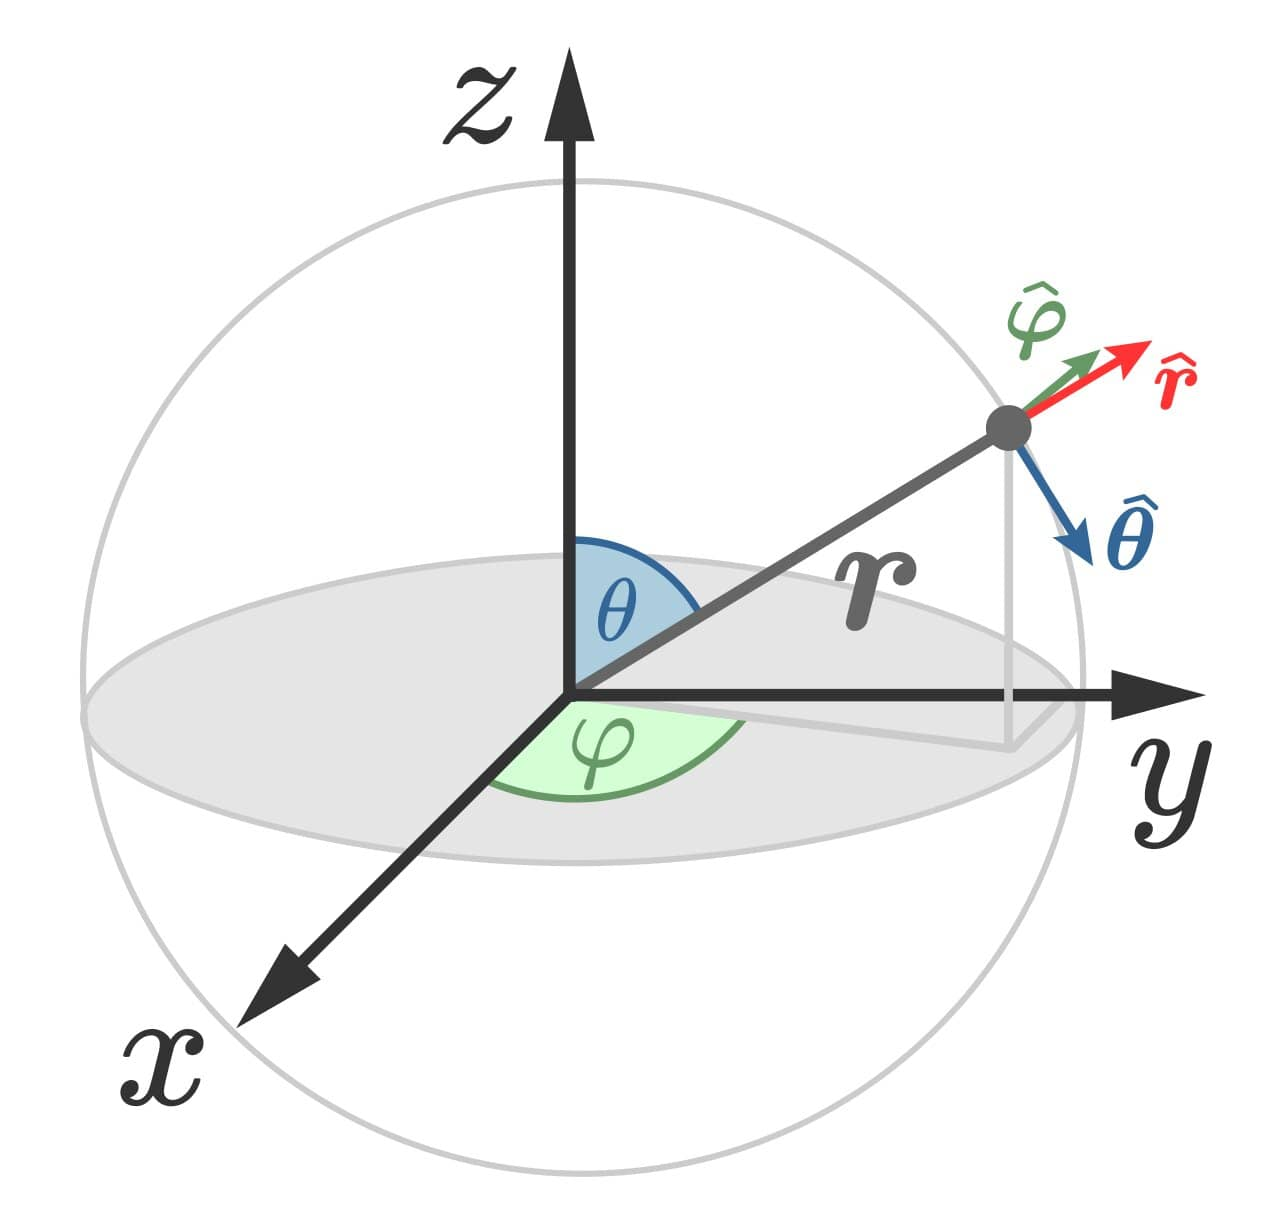
\includegraphics[width=4cm]{spherical-coordinates.jpg}
		\tiny{Quelle: universaldenker.org}\\
		\normalsize
		\subsection{Integralsätze anwenden}
		    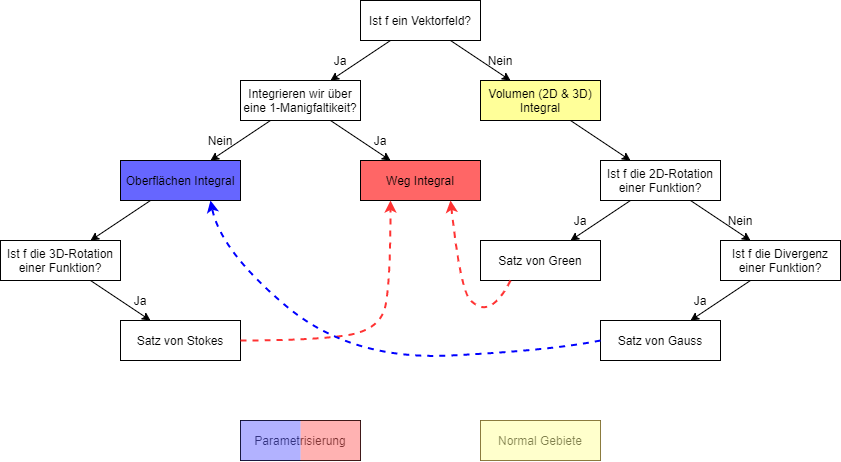
\includegraphics[scale=0.55, angle=270]{IntegralTree.png}
		    \tiny{Quelle: Analysis II PVK-Skript, Timur Locher, 2021}\\
		    \normalsize
	    \subsection{Disclaimer}
			Diese Zusammenfassung wurde für die Vorlesung Analysis I \& II im HS20 bzw. FS21 erstellt. Sie basiert auf der Zusammenfassung von Colin Dirren und Marek Landert, mit Ergänzungen von Nico Müller, Severin Nigg, Armin Riess und Robin Sieber. Der Schwerpunkt der Zusammenfassung liegt auf der Methodik und nicht auf dem mathematischen Formalismus. Es wird keine Garantie für die Richtigkeit der angegebenen Daten erteilt.
	\end{multicols*} 
\end{document}